% !TEX TS-program = pdflatexmk
\documentclass[12pt]{amsart}

%auto-ignore
%this ensures the arxiv doesn't try to start TeXing here.
%!TEX root=exceptional.tex
\usepackage{amssymb}
\usepackage{array}
\usepackage{booktabs}
\usepackage{mdwtab}
\usepackage{mathtools}
\usepackage[T1]{fontenc}
\usepackage[utf8]{inputenc}
\usepackage{libertine}
\usepackage[libertine]{newtxmath}
\usepackage{hyphenat}
\usepackage{enumitem}
\usepackage{xcolor}
\definecolor{medium-blue}{rgb}{0,0,0.65}
\usepackage{ifpdf}
\ifpdf
  \usepackage[pdftex]{graphicx}
  \usepackage[pdftex,margin=1.25in]{geometry}
  \usepackage[bookmarks=true, bookmarksopen=true,%
    bookmarksdepth=3,bookmarksopenlevel=2,%
    colorlinks=true,%
    linkcolor=purple,%
    citecolor=medium-blue,%
    filecolor=blue,%
    menucolor=blue,%
    urlcolor=medium-blue]{hyperref}
  \hypersetup{pdftitle={Towards the quantum exceptional series}}
  \hypersetup{pdfauthor={Scott Morrison, Noah Snyder, and Dylan P. Thurston}}
\else
  \usepackage[dvips]{graphicx}
  \usepackage[dvips,margin=1in]{geometry}
  % Use hyperref with all features turned off even in DVI mode, since
  % the .aux file format changes
  \usepackage[draft]{hyperref}
\fi
\usepackage{url}
\usepackage{todonotes}
\usepackage{tikz}
\usetikzlibrary{shapes}
\usetikzlibrary{calc}
\usetikzlibrary{knots}

\usepackage[backend=biber,style=alphabetic,doi=false,isbn=false,url=false,minnames=6,maxnames=6]{biblatex}
\setcounter{biburlnumpenalty}{9000}
\setcounter{biburllcpenalty}{1000}
\setcounter{biburlucpenalty}{8000}
\renewbibmacro{in:}{%
  \ifentrytype{article}{}{\printtext{\bibstring{in}\intitlepunct}}}
\renewbibmacro*{volume+number+eid}{%
  \printtext{vol.}
  \printfield{volume}%
  \setunit*{\addnbspace}% NEW (optional); there's also \addnbthinspace
  \printfield{number}%
  \setunit{\addcomma\space}%
  \printfield{eid}}
\DeclareFieldFormat[article]{number}{\mkbibparens{#1}}
\usepackage{silence}
% Filter warnings issued by package biblatex starting with "Patching footnotes failed"
\WarningFilter{biblatex}{Patching footnotes failed}
\addbibresource{bibliography/bibliography.bib}

% A binary operator with a subscript on both sides (and correct spacing)
% Name stands for subscript-operator-subscript
\newcommand{\sos}[3]{\mathbin{{}_{#1}\mathord#2_{#3}}}

% manyindices
% Adapted from code by "bza" in comp.text.tex, Feb. 7, 2006
%% USAGE:
%%
%% \manyindices#1#2#3#4#5
%%
%% #1=lower left index
%% #2=upper left index
%% #3=lower right index
%% #4=upper right index
%% #5=main symbol
\makeatletter
\newcommand\mi@kern[1]{%
  \settowidth\@tempdima{$\mi@obj^{#1}$}
  \kern-\@tempdima
  #1
  \settowidth\@tempdima{$\mi@obj$}
  \kern\@tempdima
}

\newtoks\mi@toksp
\newtoks\mi@toksb
\DeclareRobustCommand{\manyindices}[5]{
  \def\mi@obj{#5}
  \mi@toksp\expandafter{\mi@kern{#2}}
  \mi@toksb\expandafter{\mi@kern{#1}}
  \@mathmeasure4\textstyle{#5_{#1}^{#2}}
  \@mathmeasure6\textstyle{#5_{#3}^{#4}}
  \dimen0-\wd6 \advance\dimen0\wd4
  \@mathmeasure8\textstyle{\hphantom{{}_{#1}^{#2}}#5^{\the\mi@toksp#4}_{\the\mi@toksb#3}}
  \hbox to \dimen0{}{\kern-\dimen0\box8}
}
\makeatother 

% Left sub/super scripts
% \lsup is a temporary definition until something better is worked out
% Use \lsupv if the next argument is vertical
\newcommand{\lsub}[2]{{}_{#1}#2}
\newcommand{\lsup}[2]{{}^{#1}\mskip-.6\thinmuskip#2}
\newcommand{\lsupv}[2]{{}^{#1}#2}
\newcommand{\lsubsup}[3]{\manyindices{#1}{\mskip.6\thinmuskip#2\mskip-.6\thinmuskip}{}{}{\mathord{#3}}}
\newcommand{\lsubsupv}[3]{\manyindices{#1}{\mskip.2\thinmuskip#2\mskip-.2\thinmuskip}{}{}{\mathord{#3}}}

\newcounter{saveenum}

% Read the file, if it exists
\newread\testin
\def\maybeinput#1{
\openin\testin=#1
\ifeof\testin\typeout{Warning: input #1 not found}\else\input#1\fi
\closein\testin
}

\def\mathcenter#1{%
  \vcenter{\hbox{$#1$}}%
}

\def\graph#1{
        \includegraphics{#1}
}

\def\mathgraph#1{
        \mathcenter{\graph{#1}}
}

\def\mfig#1{
        \mathcenter{\includegraphics{#1}}
}

\def\mfigb#1{
        \mathcenter{\includegraphics[trim=-1 -1 -1 -1]{#1}}
}


%%% Local Variables: 
%%% mode: latex
%%% TeX-master: "main"
%%% End: 

\usepackage{fp}
\usepackage{tikz}
\usetikzlibrary{matrix}
\usetikzlibrary{arrows,backgrounds,patterns,scopes,external,hobby,
    decorations.pathreplacing,
    decorations.pathmorphing
}

\newlength{\fuzzwidth}
\setlength{\fuzzwidth}{2.5pt}
\newlength{\arrowlength}
\setlength{\arrowlength}{8pt}
\newlength{\arrowwidth}
\setlength{\arrowwidth}{.75pt}
\newlength{\pointrad}
\setlength{\pointrad}{1.5pt}
\newlength{\linewid}
\setlength{\linewid}{1.5pt}
\newlength{\circlerad}
\setlength{\circlerad}{16pt}
\newlength{\smcirclerad}
\setlength{\smcirclerad}{8pt}
\newcommand{\fillcolor}{black!60}
\newcommand{\fuzzcolor}{black!25}
\newcommand{\arrowcolor}{black!25}
\newcommand{\covercolor}{black!0}
\newcommand{\graycolor}{black!55}
\newcommand{\graylightcolor}{black!40}


\newcommand{\coverwidthfuzz}{6pt}
\newcommand{\coverwidth}{3.5pt}
\newcommand{\coverwidththin}{3.25pt}
\newcommand{\coverwidththick}{3.75pt}

\newlength{\linewidthin}
\setlength{\linewidthin}{1.25pt}
\newlength{\linewidthick}
\setlength{\linewidthick}{1.75pt}


\tikzset{use Hobby shortcut}
\tikzset{
	coverline/.style={
	preaction={draw,line width=\coverwidth,\covercolor}}, 
	coverlinethin/.style={
	preaction={draw,line width=\coverwidththin,\covercolor}}, 
	coverlinethick/.style={
	preaction={draw,line width=\coverwidththick,\covercolor}}, 
	coverlineleft/.style={
	preaction={draw,line width=\coverwidthfuzz,\covercolor,decorate,decoration={curveto,amplitude=0,raise=.35*\fuzzwidth}}}, %%% Notice this number was tweaked, 	
coverlinelefttail/.style={
	preaction={draw,line width=\coverwidthfuzz,\covercolor,decorate,decoration={curveto,amplitude=0,raise=.35*\fuzzwidth,pre=moveto,pre length=2pt}}}, %%% Notice this number was tweaked, probably will not look good if parameters change.  Again here, pre removes the raise option.
        fuzzlefttail/.style={
        preaction={draw,line width=\fuzzwidth,\fuzzcolor,decorate,decoration={curveto,pre=moveto,pre length=2pt,amplitude=0,raise=.5*\fuzzwidth}}}, %%% This does not work --- somehow pre breaks the raise function.
        linestylethin/.style={line width=\linewidthin},
        linestylethick/.style={line width=\linewidthick},
        linestylegray/.style={line width=\linewid,\graycolor},
        linestylegraylight/.style={line width=\linewid,\graylightcolor}
}
\tikzset{
        fuzzright/.style={
        preaction={draw,line width=\fuzzwidth,\fuzzcolor,decorate,decoration={curveto,amplitude=0,raise=-.5*\fuzzwidth}}},
        fuzzleft/.style={
        preaction={draw,line width=\fuzzwidth,\fuzzcolor,decorate,decoration={curveto,amplitude=0,raise=.5*\fuzzwidth}}},
        fuzzrightpre/.style={ %%% Doesn't work
        preaction={draw,line width=2pt,\fuzzcolor,decorate,decoration={curveto,amplitude=0,raise=-1pt,pre=moveto,pre length=12pt}}},
        fuzzleftpre/.style={ %%% Doesn't work
        preaction={draw,line width=2pt,\fuzzcolor,decorate,decoration={curveto,post=moveto,post length=32pt,amplitude=0,raise=1pt}}},        
        outstyle/.style={\arrowcolor, line width=\arrowwidth},
        linestyle/.style={line width=\linewid}
}

\newcommand{\lilarrow}{
\draw[->] (0,0) -- (1,0);
}

\newcommand{\cb}{\raisebox{.6ex-.5\height}}


%%%% These draw triple or quadruple set of arrows of length 0.5 cm
\DeclareMathOperator{\rightdoublearrows} {{\; 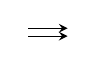
\begin{tikzpicture} \foreach \y in {0.05, 0.15} { \draw [-stealth] (0, \y) -- +(0.5, 0);} \; \end{tikzpicture}}}
\DeclareMathOperator{\leftdoublearrows} {{\; 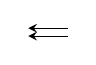
\begin{tikzpicture} \foreach \y in {0.05, 0.15} { \draw [stealth-] (0, \y) -- +(0.5, 0);} \; \end{tikzpicture}}}
\DeclareMathOperator{\righttriplearrows} {{\; 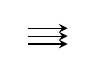
\begin{tikzpicture} \foreach \y in {0, 0.1, 0.2} { \draw [-stealth] (0, \y) -- +(0.5, 0);} \; \end{tikzpicture}}}
\DeclareMathOperator{\lefttriplearrows} {{\; 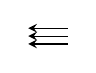
\begin{tikzpicture} \foreach \y in {0, 0.1, 0.2} { \draw [stealth-] (0, \y) -- +(0.5, 0);} \; \end{tikzpicture}}}
\DeclareMathOperator{\rightquadarrows} {{\; 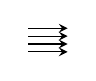
\begin{tikzpicture} \foreach \y in {-0.05, 0.05, 0.15, 0.25} { \draw [-stealth] (0, \y) -- +(0.5, 0);} \; \end{tikzpicture}}}
\DeclareMathOperator{\leftquadarrows} {{\; 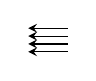
\begin{tikzpicture} \foreach \y in {-0.05, 0.05, 0.15, 0.25} { \draw [stealth-] (0, \y) -- +(0.5, 0);} \; \end{tikzpicture}}}

\newcommand{\ngon}[2][0]{
\begin{tikzpicture}[baseline=-0.5ex,scale=0.8]
\foreach \x in {1, ..., #2}
	\draw (360*\x/#2+#1:.8cm)--(360*\x/#2+#1:.5cm);
\foreach \x in {1, ..., #2}
	\draw (360*\x/#2+#1:.5cm) .. controls +(360*\x/#2+120+#1:.3cm) and +(360*\x/#2+360/#2-120+#1:.3cm) .. (360*\x/#2+360/#2+#1:.5cm);
\end{tikzpicture}
}

\newcommand{\nvertex}[2][0]{
\begin{tikzpicture}[baseline=-0.5ex,scale=0.8]
\foreach \x in {1, ..., #2}
	\draw (360*\x/#2+#1:.8cm)--(0,0);
\end{tikzpicture}
}

\newcommand{\unknot}{
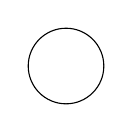
\begin{tikzpicture}[baseline=-0.5ex,scale=0.8]
  \draw (0,0) circle (.6cm);
\end{tikzpicture}
}

\newcommand{\drawI}{ 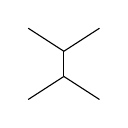
\begin{tikzpicture}[baseline=-0.5ex,scale=0.8]
 	\draw (0,.2) -- (45:.8cm);
 	\draw (0,.2) -- (135:.8cm);
	\draw (0,.2) -- (0,-.2);
 	\draw (0,-.2) -- (-45:.8cm);
 	\draw (0,-.2) -- (-135:.8cm);
\end{tikzpicture}
}

\newcommand{\drawH}{ 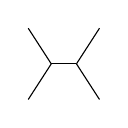
\begin{tikzpicture}[baseline=-0.5ex,rotate=90,scale=0.8]
 	\draw (0,.2) -- (45:.8cm);
 	\draw (0,.2) -- (135:.8cm);
	\draw (0,.2) -- (0,-.2);
 	\draw (0,-.2) -- (-45:.8cm);
 	\draw (0,-.2) -- (-135:.8cm);
\end{tikzpicture}}

\newcommand{\onestrandid}{\begin{tikzpicture}[baseline=-0.5ex,scale=0.8]
	\draw (-.8cm,0)--(.8cm,0);
\end{tikzpicture}}

\newcommand{\twostrandid}{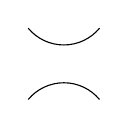
\begin{tikzpicture}[baseline=-0.5ex,scale=0.8]
	\draw (45:.8cm) to [curve through=(90:.3cm)] (135:.8cm);
	\draw (-45:.8cm) to [curve through=(-90:.3cm)] (-135:.8cm);
\end{tikzpicture}}

\newcommand{\cupcap}{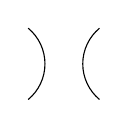
\begin{tikzpicture}[baseline=-0.5ex,rotate=90,scale=0.8]
	\draw (45:.8cm) to [curve through=(90:.3cm)] (135:.8cm);
	\draw (-45:.8cm) to [curve through=(-90:.3cm)] (-135:.8cm);
\end{tikzpicture}}

\newcommand{\symcross}{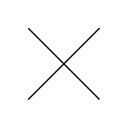
\begin{tikzpicture}[baseline=-0.5ex,scale=0.8]
	\draw (45:.8cm) -- (-135:.8cm);
	\draw (-45:.8cm) -- (135:.8cm);
\end{tikzpicture}}

\newcommand{\braidcross}{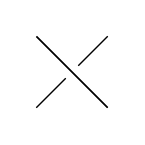
\begin{tikzpicture}[baseline=-0.5ex,scale=0.8]
	\draw (45:.8cm) -- (-135:.8cm);
	\draw[line width=1mm,white,double=black] (-45:.8cm) -- (135:.8cm);
\end{tikzpicture}}


\newcommand{\drawcrossX}{ 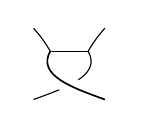
\begin{tikzpicture}[baseline=-0.5ex,scale=0.8,rotate=90]
 	\draw ([out angle=30].2,.3) .. (45:.8cm);
	\draw (.2,.3) -- (.2,-.3);
 	\draw ([out angle=-30].2,-.3) .. (-45:.8cm);
        \draw ([out angle=-150].2,-.3) ..([in angle=-70]135:.8cm);
 	\draw[line width=1mm,white,double=black]
              ([out angle=150].2,.3) .. ([in angle=70]-135:.8cm);
\end{tikzpicture}}

\newcommand{\twist}{
  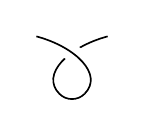
\begin{tikzpicture}[baseline=-0.5ex,scale=0.8]
    \draw[line width=1mm,white,double=black]
       ([out angle=-15]135:.8cm)..([blank=soft]-60:.4cm)..(-120:.4cm)..([in angle=-165]45:.8cm);
    \draw[line width=1mm,white,double=black,use previous Hobby path={invert soft blanks,disjoint}];
  \end{tikzpicture}}

\newcommand{\twistvertex}{
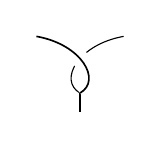
\begin{tikzpicture}[baseline=-0.5ex,scale=0.8]
  \draw (0,-0.5)--(0,-0.8);
  \draw ([out angle=-170]30:0.8cm)..([in angle=150](0,-0.5);
  \draw[line width=1mm,white,double=black]
        ([out angle=-10]150:0.8cm)..([in angle=30](0,-0.5);
\end{tikzpicture}}

\newcommand{\loopvertex}{
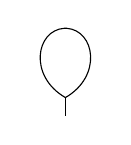
\begin{tikzpicture}[baseline=-0.5ex,scale=0.8]
  \draw (0,-0.5)--(0,-0.8);
  \draw ([out angle=150]0,-0.5)..(-0.02,0.6)..(0.02,0.6)..([in angle=30]0,-0.5);
\end{tikzpicture}
}

\newcommand{\pentagon}{
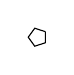
\begin{tikzpicture}[scale=.12,baseline=-2]
\draw (36:1) -- (108:1) -- (180:1) -- (252:1) -- (-36:1) -- (36:1);
\end{tikzpicture}
}

\newcommand{\psq}{
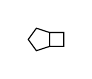
\begin{tikzpicture}[scale=.15,baseline=-2]
\draw (36:1) -- (108:1) -- (180:1) -- (252:1) -- (-36:1) -- (36:1) -- +(1.2,0) -- ($(-36:1)+(1.2,0)$) -- (-36:1);
\end{tikzpicture}
}

\newcommand{\sqsq}{
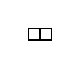
\begin{tikzpicture}[scale=.15]
\draw (0,0) -- (2,0) -- (2,1) -- (0,1) -- cycle (1,0) -- (1,1);
\end{tikzpicture}
}


\begin{document}
\title{Towards the quantum exceptional series}

\author[Morrison]{Scott~Morrison}
\address{Mathematical Sciences Institute, Australian National University}
\email{scott.morrison@anu.edu.au}

\author[Snyder]{Noah~Snyder}
\address{Bloomington, Indiana, USA}
\email{nsnyder1@indiana.edu}

\author[Thurston]{Dylan~P.~Thurston}
\address{Bloomington, Indiana, USA}
\email{dpthurst@indiana.edu}

\begin{abstract}
  We find a single two-parameter skein relation on trivalent graphs,
  the \emph{quantum exceptional relation}, that specializes to a skein
  relation associated to each exceptional Lie algebra (in the adjoint
  representation). If a slight
  strengthening of Deligne's conjecture on the existence of a
  (classical) exceptional series is true, then this relation
  holds for a new two-variable quantum exceptional polynomial, at
  least as a power series near $q=1$. The
  single quantum exceptional relation implies both the
  Jacobi relation (true for every Lie algebra) and
  the Vogel relation holding for the exceptional series.

  We find a conjectural basis for the space of diagrams with $n$ loose
  ends modulo the quantum exceptional relation for $n \le 7$, with
  dimensions agreeing with the classical computations, and compute
  the matrix of inner products. \nn{(Dimensions of idempotents?)}
  We use the
  skein relation to compute the conjectural quantum exceptional
  polynomial for many knots, in particular
  determining (unconditionally) the values of the quantum polynomials
  for the exceptional Lie algebras on
  these knots. The knots we can compute for include all knots with up
  to 11 (12?) crossings.
\end{abstract}

%\subjclass[2000]{Primary xxx; Secondary xxx}
%\keywords{}

\maketitle

\tableofcontents

A proposed new outline:
\begin{enumerate}
\item Introduction
\begin{enumerate}
\item Two-variable knot polynomials. For a two-variable knot polynomial to
exist, we first need a family of Lie algebras, and second need a coherent
quantisation of the family. We propose that this can be achieved in the 
exceptional series, and give many calculations of the conjectured knot
invariant.
\item Deligne's classical exceptional series, generators, relations, and 
conjectures.
\item The main result of this paper is a conjecture.
The quantum exceptional series, generators and relations and conjectures.
\item The rest of the paper consists of two kinds of evidence for this 
conjecture.
\begin{enumerate}
\item First, we show that the proposed description of the quantum exceptional 
series is the right one --- it is picked out as the unique braided tangle
category
with ...
\item Second, we give some weak evidence that the conjecture is viable.
\begin{enumerate}
\item We propose bases for the $n$-box spaces, $n \leq 6$ (or is it 7?), 
showing that these are linear independent, and their spans are closed under
various operations.
\item We show that these give representations of the affine $n$-strand braid 
groups, for $n \leq 6$.
\item We calculate ridiculously many two-variable knot polynomials; although 
these are conjectural, they unconditionally specialise to the correct quantum
knot polynomials for the exceptional Lie algebras.
\end{enumerate}
\item Mention the Kontsevich integral argument?
\end{enumerate}
\end{enumerate}
\item Main results
\begin{enumerate}
\item The classification statement.
\item We defer some corner cases to the end.
\item Proof of the main case.
\item Statement of the evaluation and consistency conjectures.
\item Some consequences: other relations.
\item Specializations.
  \begin{enumerate}
  \item $U_q(\fg)$ for $\fg$ in Deligne's list in the adjoint
    representation
  \item The 7-dimensional representation of $U_q(\fg_2)$
  \item $U_q(\fg)$ for $\fg$ in the $F_4$ family
    At $q=1$, these have $v^6=-1$ (since the trivalent vertex is
    symmetric). This family has only a finite number of points.
  \end{enumerate}
\end{enumerate}
\item Calculations
\begin{enumerate}
\item Heuristics for choosing bases for $n$-box spaces
\item Verifying linear independence, and invariance under operations
\item A representation of the affine 6-strand braid group
\item 2-variable polynomials for knots with Conway width at most 6.
\begin{enumerate}
\item Define Conway graph and Conway width.
\item Explain that we can calculate anything with Conway width at most 6.
\item This includes all 12-crossing knots, and all but one 12-crossing link.
\item Mention Westbury's paper, and the other paper that has done some knot
polynomial calculations.
\end{enumerate}
\item Denominators.
\item Dimensions of irreducible objects.
\end{enumerate}
\item A Kontsevich integral argument: the classical conjecture implies the
quantum conjecture.
\item Corner cases from the classification.
\end{enumerate}



\section{Introduction}
\label{sec:introduction}

There are two main 2-variable knot polynomials: the HOMFLY-PT polynomial and
the Kauffman polynomial.  The HOMFLY-PT polynomial interpolates between the
Reshetikhin--Turaev invariants of the standard representations of
$U_q(\mathfrak{gl}_n)$, while the Kauffman polynomial does the same for the
standard representations of quantum $U_q(\mathfrak{o}_n)$ (or, in a slightly
different form, the standard representations of $U_q(\mathfrak{sp}_n)$).  The
two variable nature of these knot polynomials come from the two parameters $n$
and $q$, but we need to replace the discrete parameter $n$ with a continuous
one.   One can think of this process in two steps: first construct a family of
Lie algebra objects in symmetric tensor categories which interpolate between
the $\mathfrak{gl}_n$ yielding something called $\mathfrak{gl}_t$, and second
quantize these Lie algebra objects.   This quantization can be done
systematically using the Kontsevich integral, provided it converges.

Work of Deligne, Cvitanović, Vogel, Cohen-de Man, and others, can be
summarized as a conjecture that there is a third 1-parameter family of Lie
algebra objects in symmetric tensor categories, called the (classical)
exceptional series. This should interpolate between the adjoint
representations of $\mathfrak{sl}_2$, $\mathfrak{sl}_3$, $\mathfrak{so}_8$,
$\mathfrak{g}_2$, $\mathfrak{f}_4$, $\mathfrak{e}_6$, $\mathfrak{e}_7$, and
$\mathfrak{e}_8$ in an appropriate sense.  If this classical exceptional
family exists, we should again expect a quantization yielding a 2-variable
exceptional knot polynomial.  In this paper we give a conjectural skein
theoretic description of this exceptional knot polynomial. In fact, we prove
that these particular skein relations must hold if the exceptional knot
polynomial exists.

We can use these skein relations to do many computations.  In particular, we
are able to calculate the value of this knot polynomial (if it exists!) on all
knots of Conway girth 6, which includes all knots of 12 or fewer crossings.
Unconditionally these give the first calculations of the Reshetikhin-Turaev
knot invariants for the exceptional Lie algebras for most of these knots.  For
example, we compute the following value for the trefoil for the exceptional
series, and the Reshetikhin-Turaev invariant for $\mathfrak{e}_8$ is given by
setting $v=q^5$ and $w=q^6$.
\begin{multline*}
QES_{\text{reduced}}(\nn{trefoil}) = \\
-v^{24}
\Big(
    \left(w^4 + v^4 w^{-4}\right)\left(-v^{22}+v^{12}+v^{10}-1\right)+\\
    \left(w^2 + v^2 w^{-2}\right)\left(-v^{34}+v^{30}-v^{26}+v^{24}+v^{22}-v^{20}-v^{18}+v^{16}+v^{14}-v^{12}+v^8-v^4\right)+\\
    \left(v^{36}+v^{34}-v^{32}+v^{28}-3 v^{24}-v^{22}+2 v^{20}-v^{16}+v^{14}+2 v^{12}-v^8-v^2-1\right)
    \Big)
\end{multline*}

We are also able to do several other calculations, like giving quantum
dimension formulas for the summands of $\mathfrak{g}^{\otimes 3}$ quantizing
the dimension formulas of Cohen--De Man \cite{MR1381778} in the classical case
(for the summands of $\mathfrak{g}^{\otimes 2}$ such quantum dimension
formulas were already given by Tuba-Wenzl \cite{MR2132671}).

In order to state these conjectures and theorems precisely and place them in
their proper context, we have written a  long introduction split into several
subsections.

\subsection{The classical exceptional series}
In order to motivate our results about the quantum exceptional series, we will
give precise statementsof some conjectures giving a skein theoretic
description of the classical exceptional series following Cvitanovic, Deligne,
and Vogel.

We begin with the symmetric tensor category of Jacobi
diagrams, $\mathrm{Jac}_d$.

\begin{definition}
Let $R$ be an algebra over $\mathbb{C}$, and let $d$ be an element of $R$ and
$b$ an invertible element of $R$.  The objects of $\mathrm{Jac}_{R,d,b}$ are
collections of $n$ points on the line and the morphism space from $n$ to $m$
consists of $R$-linear combinations of planar graphs in a rectangle with $n$
boundary points on the bottom, $m$ boundary points at the top, and consisting
of trivalent vertices and $4$-valent symmetric crossings
\DPTtodo{Expand on ``symmetric crossing''}
modulo planar isotopy, the usual Reidemeister 2 and 3
relations for a symmetric crossing, and the following circle, lollipop, bigon,
triangle, anti-symmetry, symmetry of the Killing form, and Jacobi relations.

\begin{align}
\label{eq:classical-loop-lollipop}  \unknot \; &= d &  \loopvertex \; &=0 \\
\label{eq:classical-bigon-trigon}  \ngon{2}\; &= b \;\onestrandid  & \ngon{3}\; &= \frac{b}{2} \;\nvertex{3} \\
\label{eq:classical-symmetry-antisymmetry}   \symtwistvertex\; &= - \nvertex[-90]{3} & \symtwist\; &= \drawcup
\end{align}
\begin{equation}
\drawI\; - \;\drawH\; + \;\drawsymcrossX\; = 0.
\label{eq:IHX}
\end{equation}
\end{definition}

By rescaling the trivalent vertex, it is easy to see that
$\mathrm{Jac}_{R,d,b}$ is equivalent as a spherical tensor category to
$\mathrm{Jac}_{R,d,bx^2}$ for any invertible $x$ in $R$.  In particular, if $R
= \mathbb{C}$ then $\mathrm{Jac}_{R,d,b}$ does not depend on the choice of
$b$.  A standard normalization is $b=6$.
\NStodo{Should we change $6$ to $12$?}

If $\mathfrak{g}$ is a simple Lie algebra object in a symmetric tensor
category with dimension $d$, by the diagram calculus  the symmetric tensor
category of finite dimensional representations of $\mathfrak{g}$ is the target
of a functor from $\mathrm{Jac}_{R,d,b}$, where we interpret each strand as a
copy of $\mathfrak{g}$, each cup or cap using the Killing form, each trivalent
vertex as the Lie bracket, and each crossing as the usual symmetric braiding.
This  skein theory is somewhat poorly behaved since the space of $0$-boundary
point diagrams is expected to be infinite dimensional.

In addition, Cvitanović and Vogel independently observed that the adjoint
representations of the exceptional Lie algebras satisfy another relation, the
\emph{classical exceptional relation}.

\begin{definition}
If $2+d$ is invertible in $R$, let $\mathrm{Exc}_{R,d,b}$ be symmetric tensor category which is the quotient of 
$\mathrm{Jac}_{R,d,b}$ modulo the exceptional relation.
\begin{equation}
\ngon[45]{4}\; = \frac{b}{6} \left(\;\drawI\; + \;\drawH\; \right)
 + \frac{5}{6}\frac{b^2}{2+d} \left( \;\cupcap\; + \;\twostrandid\; + \;\symcross\; \right)
\label{eq:classical-except}
\end{equation}
\end{definition}

The parameter $d$ is somewhat poorly behaved, and so Deligne instead
introduced a parameter $\lambda$ such that $d = -2
\frac{(\lambda+5)(6-\lambda)}{\lambda(1-\lambda)}$.  This makes sense so long
as $\lambda$ and $1-\lambda$ are invertible in $R$, and such a $\lambda$ can
be found when $2+d$ is invertible and $(2+d)(242+d)$ has a square root in $R$.
Note that $\lambda$ and $1-\lambda$ correspond to the same $d$ and thus to the
same category.  If we normalize $b=6$ then the exceptional relation for
$\mathrm{Exc}_{R,-2   \frac{(\lambda+5)(6-\lambda)}{\lambda(1-\lambda)},6}$
(which we will also write $\mathrm{Exc}_{R,\lambda}$) has the following form.

\begin{equation}
\ngon[45]{4}\; = \;\drawI\; + \;\drawH\;
 - \frac{\lambda(1-\lambda)}{2} \left( \;\cupcap\; + \;\twostrandid\; + \;\symcross\; \right)
\label{eq:classical-except-2}
\end{equation}


\begin{conjecture}[Classical sufficiency]
  \label{conj:class-suffic}
So long as a certain finite set of polynomials in $\lambda$ are invertible,
the space of $n$-boundary point diagrams in $\mathrm{Exc}_{R,\lambda}$ is
finitely generated as an $R$-module for every $n$.  Furthermore,
$\mathsf{Exc}_{R,\lambda}(0,0)$ is generated by the empty diagram,
$\mathsf{Exc}_{R,\lambda}(1,0)$ is the $0$-module,
$\mathsf{Exc}_{R,\lambda}(1,1)$ is spanned by the strand,
$\mathsf{Exc}_{R,\lambda}(2,1)$ is spanned by the trivalent vertex, and
$\mathrm{Exc}_{R,\lambda}(2,2)$ is generated by $$\symcross\;, \; \drawI \;,
\; \drawH \;, \; \twostrandid \;, \text{ and } \; \cupcap \; .$$
\end{conjecture}

We also conjecture specific spanning sets for $\mathsf{Exc}_{R,\lambda}(n,m)$
for $n+m \leq 6$, see Section~\ref{sec:bases}.

\begin{conjecture}[Classical consistency]
  \label{conj:class-consist}
So long as a certain finite set of polynomials in $\lambda$ are invertible in
$R$, then $R$ injects into $\mathrm{Exc}_{R,\lambda}(0,0)$ as multiples of the
empty diagram.  In particular, any two ways of simplifying the same closed
diagram to give an element of $R$ will give the same element of $R$.
\end{conjecture}

Note that if $d$ is invertible in $R$, it follows from classical consistency
that $R$ injects into $\mathrm{Exc}_{R,\lambda}(1,1)$ as multiples of the
strand.  Similarly if $b$ and $d$ are invertible in $R$, it follows from
classical consistency that $R$ injects into $\mathrm{Exc}_{R,\lambda}(2,1)$ as
multiples of the trivalent vertex  Similarly, if \NStodo{what polynomials?}
are invertible, then $R^4$ injects into $\mathrm{Exc}_{R,\lambda}(2,2)$ as
linear combinations of the above four diagrams.

\nn{Do we have any speculations about what elements of $R$ need to be inverted.}

If both consistency and sufficiency hold, it is also natural to conjecture
that $\mathrm{Exc}_{R,\lambda}(n,m)$ is always a free $R$-module of finite
rank.  When $n+m$ is small this follows from our calculations and the above
conjectures.

\begin{corollary}[Classical specialization]
If Conjecture \ref{conj:class-suffic} and $\lambda$ is one of $$-5, -4, -3,
-2, -3/2,-1,-2/3,-1/2,-1/3,-1/5,$$ then the quotient of
$\mathrm{Exc}_{\mathbb{C},\lambda}$ by the negligible elements is equivalent
to the category of representations of the following compact supergroups: the
trivial group, $\mathrm{OSp}(1 | 2)$, $\mathrm{PSL}(2)$, $\mathrm{PSL}(3)
\rtimes \mathbb{Z}/2$, $G_2$, $\mathrm{PO}(8) \rtimes \mathbb{Z}/3$, $F_4$,
$E_6 \rtimes \mathbb{Z}/2$, $E_7$, and $E_8$, respectively.
\end{corollary}

Here's a rough sketch of the proof given in Section ??? (some modification is
needed for $\mathrm{OSp}(1|2)$).  All the skein relations in
$\mathrm{Exc}_{\mathbb{C},\lambda}$ do hold in the corresponding
representation categories, so we get a functor which is injective on morphisms
and essentially surjective on objects.  By Tannaka--Krein duality and
unitarity, the image of this functor is the category of representations of a
compact subgroup of $\mathrm{U}(\ad)$ preserving the bracket and containing
the group.  But each of these groups is the maximal such unitary group
preserving the bracket, so the functor is surjective on morphisms.

\NStodo{Is this nonsense?}

\DPTtodo{What is $\mathrm{U}(\ad)$, and does this kind of detail
  belong here??}

\begin{conjecture}[Classical semisimplicity]
There is a dense open subset $U \subset \mathbb{C}$ for which the idempotent
completion of $\mathrm{Exc}_{\mathbb{C},\lambda}$, for $\lambda \in U$, is
semisimple.
\end{conjecture}

We expect that in order for the idempotent completion to be semisimple one
needs to invert infinitely many polynomials.  For example, for the idempotent
completion of $\mathrm{GL}_t$ to be semisimple you need to invert $t-n$ for
every positive integer $n$.  From the dimension formulas of Cohen--De Man and
others, we might speculate that for classical semisimplicity it is again
enough to invert $\lambda-n$ for $n \in \mathbb{Z}$.

These conjectures are a strengthening of a the conjecture of Deligne (as
improved by Cohen--De Man who incorporated the Cvitanović--Vogel exceptional
relation), and would give a construction of an exceptional series passing
through each of the exceptional Lie algebras.

\begin{conjecture}[Deligne's conjecture]
There exists
  \begin{itemize}
  \item a ring $R$ which is a localization of $\mathbb{C}[\lambda]$ at finitely many polynomials
  \item a category $\mathsf{Except}_{R,\lambda}$ where the objects are integers and morphism spaces are finitely-generated $R$-modules.
  \item a braided functor $\eval$ from $\mathsf{Exc}_{R,\lambda}$ to $\mathsf{Except}_{R,\lambda}$, that is the identity on objects and surjective on morphisms and sends the trivalent vertex to the generator of the $3$-boundary point space. 
  \end{itemize}
For any map $\varphi: R \rightarrow S$ we can define the base extension $\mathsf{Except}_{S,\varphi(\lambda)}$.  Furthermore $\mathsf{Except}$ has the following properties
\begin{itemize}
\item the idempotent completion of $\mathsf{Except}_{\mathbb{C}(\lambda),\lambda}$ is semisimple.
\item $\mathsf{Except}_{\mathbb{C}(\lambda),\lambda}(n,m)$ has dimension $1,\allowbreak0,\allowbreak1,\allowbreak1,\allowbreak5,\allowbreak16,\allowbreak80$
for $n+m=0,1,2,3,4,5,6$, respectively, 
\item if $\lambda$ is one of $-5, -4, -3, -2, -3/2,-1,-2/3,-1/2,-1/3,-1/5$, then the quotient of $\mathrm{Exc}_{\mathbb{C},\lambda}$ by the negligible elements is equivalent to the category of representations of the trivial group, $O(1 | 2)$, $\mathrm{PSL}(2)$, $\mathrm{PSL}(3) \rtimes \mathbb{Z}/2$, $G_2$, $\mathrm{PO}(8) \rtimes \mathbb{Z}/3$, $F_4$, $E_6 \rtimes \mathbb{Z}/2$, $E_7$, and $E_8$, respectively.
\end{itemize}
\end{conjecture}

\DPTtodo{Add note: Vogel believes Deligne's conjecture is false}

Our conjectures imply Deligne's conjecture for $\mathsf{Except}_{R,\lambda} =
\mathsf{Exc}_{R,\lambda}$, so they are slightly stronger and say that the
classical exceptional relation is the only skein relation needed to define
$\mathsf{Except}_{R,\lambda}$.

\subsection{Some Laurent polynomial conventions}

The main result of this paper is a quantum versions of the sufficiency and
consistency conjectures.   Before stating these conjecture we fix some
notation for certain Laurent polynomials appearing in our formulas.  On the
one hand, we would like to use formulas that are irreducible as Laurent
polynomials in $v$ and $w$, so that we can easily read off from formulas which
primes need to be inverted.  On the other hand the Laurent polynomials that
occur in our formulas are often even or odd under $v \rightarrow v^{-1}, w
\rightarrow w^{-1}$, so we would also like our formulas to have this symmetry.
So we often combine two irreducible factors into a single expression.  For
example, $v-v^{-1} = v^{-1}(v-1)(v+1) =
(v^{\frac{1}{2}}-v^{-\frac{1}{2}})(v^{\frac{1}{2}}+v^{-\frac{1}{2}})$ but
there is no way to factor it into odd or even Laurent polynomials so we will
leave $v-v^{-1}$ alone in our formulas.  This will never cause any confusion
since any time the irreducible factor $(v-1)$ appears it will have a
corresponding $(v+1)$ factor.

\begin{align*}
[k\lambda + n] &= w^kv^n - w^{-k}v^{-n}\\
\{k\lambda + n\} &= w^k v^n + w^{-k} v^{-n}
\end{align*}

\begin{warning}
Note that, unlike with the usual quantum numbers, there is no denominator.
\end{warning}

Note that $\{k\lambda + n\}$ is always irreducible, while $[k\lambda +
n]$ is a product of two irreducibles so long as $k$ and $n$ are
relatively prime.  When
$k=0$ we will avoid $[n]$ and instead factor into the following
symmetrized cyclotomic polynomials.  (Strictly speaking we should use
a similar convention for factoring $[k \lambda]$, but this will not be
necessary.)  Let
\DPTtodo{I still object to this notation}
\[
  \widetilde{\Phi}_n = \prod_{\zeta: (\pm \zeta)^n = 1 \text{ and } (\pm \zeta)^m \neq 1 \text{ for $m < n$}}
  (v^{\frac{1}{2}}-\zeta v^{-\frac{1}{2}}).
\]
In terms of the usual cyclotomic polynomials we have if $n$ is odd
then $\widetilde{\Phi}_n = \widetilde{\Phi}_{2n} = v^{-\varphi(n)}
\Phi_n(v) \Phi_{2n}(v)$, but if $n$ is a multiple of $4$ then
$\widetilde{\Phi}_n = v^{-\frac{\varphi(n)}{2}} \Phi_n(v)$. In particular, when $n$ is odd $\widetilde{\Phi}_n$ vanishes exactly at primitive $n$-th and primitive $2n$-th roots of unity, while when $n$ is a multiple of 4, $\widetilde{\Phi}_n$ vanishes exactly at primitive $n$-th roots of unity.
The notation $\{k\lambda + n\}$ can be viewed as another case of this:
for $n$ odd,
$\{n\} = \widetilde{\Phi}_{4n}(v)$.


\subsection{Quantum exceptional conjectures}

We now turn to our main conjectures.  Our first goal is to give a definition
of a tensor category $\mathrm{QExc}$ which looks like a quantum deformation of
$\mathrm{Exc}$, in particular we need skein relations which deform the Jacobi
relation, the classical exceptional relation, and the symmetric relation
between the overcrossing and undercrossing.  Our specific choices of relations
will be motivated below by our main theorems.

\begin{definition}
Let $R$ be a ring and $v$ and $w$ invertible elements of $R$ such that
$[\lambda]$, $[\lambda-1]$, $\widetilde{\Phi}_1$, and $\widetilde{\Phi}_{12}$
are invertible. \SMtodo{write these out, just here} Let
$\mathrm{QExc}_{R,v,w}$ be the ribbon category whose objects are collections
of $n$ points on a line, and whose morphisms spaces from $n$ to $m$ consist of
$R$-linear combinations of planar graphs in a rectangle with $n$ boundary
points on the bottom, $m$ boundary points at the top, and consisting of
trivalent vertices and $4$-valent braided crossings modulo planar isotopy, the
usual Reidemeister 2 and 3 relations for a symmetric crossing, and the
following circle, lollipop, bigon, triangle, quantum anti-symmetry, and
quantum Killing symmetry relations.

 \begin{equation}
    \label{eq:simple-rels-spec}
  \begin{aligned}
    \unknot\; &= d&\quad
    \loopvertex\;&=0\\[5pt]
      \ngon{2}\;&= b\;\onestrandid&
        \ngon[-90]{3}\; &= t\;\nvertex[-90]{3}\\[5pt]
    \twistvertex\; &= -v^{6}\;\nvertex[-90]{3}&
      \twist\; &= v^{12}\;\drawcup
  \end{aligned}
  \end{equation}
where
\begin{align*}
  d &= -\frac{\widetilde{\Phi}_8 [\lambda+5][\lambda-6]}{[\lambda][\lambda-1]}\\
  b &= \{\lambda+2\}\{\lambda-3\}\widetilde{\Phi}_3\\
  t &= \widetilde{\Phi}_1 \bigl(\widetilde{\Phi}_1 \{2\lambda -1\} + (v^4 - v^2 - 1 - v^{-2} + v^{-4})\bigr).
\end{align*}


To these skein relations, we add three more relations:
\begin{itemize}
\item the \emph{quantum exceptional Jacobi relation} (QEJacobi)
\begin{equation}
v^{-3} \;
\drawcrossX
\;+ v \;
\drawI
\; -v^{-1} \;
 \drawH
\;
 - \frac{[\lambda][\lambda-1]}{\widetilde{\Phi}_1}
\left[\; \braidcross \;
 + v^{4}\;
\cupcap
\; + v^{-4} \;
 \twostrandid \;
 \right] = 0.\label{eq:quant-except-spec}
\end{equation}

\item the \emph{quantum exceptional square relation} (QESquare)

\begin{equation}
\label{eq:QESquare-w}
\ngon[45]{4} + \frac{-\widetilde{\Phi}_4\widetilde{\Phi}_{12}^2[\lambda][\lambda-1]}{\widetilde{\Phi}_1^2} \braidcross + \frac{x_1}{\widetilde{\Phi}_1} \drawI + \frac{x_2}{\widetilde{\Phi}_1} \drawH + \frac{x_3}{\widetilde{\Phi}_1^2} \cupcap + \frac{x_4}{\widetilde{\Phi}_1^2} \twostrandid =0
\end{equation}

where the $x_i$ are Laurent polynomials in $v$ and $w$ from Appendix \ref{app:coefficients}.

\item the \emph{quantum exceptional crossing relation} (QECrossing)

\begin{equation}
\label{eq:QECrossing-w}
\braidcross - \invbraidcross + \frac{\widetilde{\Phi}_1}{\widetilde{\Phi}_{12}} \left[\; \drawI \; - \; \drawH \; \right] + \frac{\widetilde{\Phi}_1 [\lambda][\lambda-1]}{\widetilde{\Phi}_{12}} \left[\; \twostrandid \; - \; \cupcap \; \right] = 0
\end{equation}


\end{itemize}
\end{definition}

Note that if you set $w = v^\lambda$ and take the limit $v \rightarrow 1$
these relations recover the classical Jacobi relation, classical exceptional
relation, and the symmetric crossing relation.  In order to make this
specialization process purely algebraic, we would need to introduce a larger
ring with formal symbols for expressions like $\frac{w-w^{-1}}{v-v^{-1}}$.

\begin{warning}
Although the quantum exceptional Jacobi relation looks like an
analogue of the ordinary Jacobi relation with lower order terms, it is
important to emphasize that it is only the correct analogue of the Jacobi
relation in the exceptional setting.  In particular, it does not hold for
quantizations of non-exceptional Lie algebras.
\end{warning}

We now state our main conjectures.

\begin{conjecture}[Quantum sufficiency]
  \label{conj:quant-suffic}
There is a finite set of polynomials in $v$ and $w$, so that if these
polynomials are invertible in $R$ then the space of $n$-boundary point
diagrams in $\mathrm{QExc}_{R,v,w}$ is finitely generated as an $R$-module for
every $n$.  Furthermore, $\mathrm{QExc}_{R,v,w}(0,0)$ is generated by the
empty diagram, $\mathrm{QExc}_{R,v,w}(0,1)$ is the zero module,
$\mathrm{QExc}_{R,v,w}(1,1)$ is generated by the strand,
$\mathrm{QExc}_{R,v,w}(2,1)$ is generated by the trivalent vertex, and
$\mathrm{QExc}_{R,v,w}(2,2)$ is generated by
$$\braidcross\;, \; \drawI \;, \; \drawH \;, \; \twostrandid \;, \text{and} \; \cupcap \; .$$
\end{conjecture}

\SMtodo{perhaps we should include a guess for these sets of polynomials}

As before we have conjectured spanning sets for $\mathsf{QExc}_{R,v,w}(n,m)$
for $n+m=0,1,2,3,4,5,6$.

\begin{conjecture}[Quantum consistency]
  \label{conj:quant-consist}
There is a finite set of polynomials in $v$ and $w$, so that if these
polynomials are invertible in $R$ then $R$ injects into
$\mathrm{QExc}_{R,v,w}$ as multiples of the empty diagram.  In particular, any
two ways of applying the above relations to a closed diagram to return a
rational function in $v$ and $w$ will yield the same rational function.
\end{conjecture}

\SMtodo{this is going to require quite a bit of unpacking: what is $q$ in
\terms of $v$, what do the semidirect products mean. We should probably
\include a later section and just refer forward for this.}

As in the classical case, we again get that if $d$ (resp. $b$) is invertible,
then $R$ also injects into $\mathrm{QExc}_{R,v,w}(1,1)$ (resp.
$\mathrm{QExc}_{R,v,w}(1,2)$) as multiples of the strand (resp. trivalent
vertex).

\begin{conjecture}[Quantum specialization]
If $\lambda$ is one \SMtodo{make a table!} of $-5, -4, -3, -2, -3/2,1,2/3,1/2,
1/3, 1/5$, and $v$ is not a root of unity, then the quotient of
$\mathrm{QExc}_{\mathbb{C},v,v^\lambda}$ by the negligible elements is
equivalent to the category of representations of the quantum versions of
trivial group, $O(1 | 2)$, $\mathrm{PSL}(2)$, $\mathrm{PSL}(3) \rtimes
\mathbb{Z}/2$, $G_2$, $\mathrm{PO}(8) \rtimes \mathbb{Z}/3$, $F_4$, $E_6
\rtimes \mathbb{Z}/2$, $E_7$, and $E_8$, respectively.
\end{conjecture}




\NStodo{Make ``quantum versions" more precise}
\SMtodo{say what little we can about $v$ a root of unity}

\begin{conjecture}[Quantum semisimplicity]
There is a dense open subset $U \subset \mathbb{C}$ for which the idempotent completion of $\mathrm{QExc}_{\mathbb{C},v,w}$, for $v,w \in U$, is semisimple.
\end{conjecture}

\NStodo{Could make more precise: $v$ not a root of unity and $w$ in $U$}


The following theorems justify the definition of the $\mathrm{QExc}$.  Under
some mild assumptions, any trivalent ribbon category where the $n$-box space
has dimension at most $1,0,1,1,5$ for $n=0,1,2,3,4$ satisfies a version of
relation QEJacobi.  Furthermore, again under some mild assumptions, the
QEJacobi relation implies QESquare and QECrossing.

%With some mild assumptions on the base ring, any skein theory where the $n$-box space has dimension at most $1,0,1,1,5$ for $n=0,1,2,3,4$ satisfies a version of relation~\eqref{eq:quant-except-spec}. %See Theorem~\ref{thm:quant-except} in Section~\ref{sec:relation} for a precise statement.

\begin{definition}
A \emph{trivalent ribbon} category $(\cC, X, \tau)$ is a ribbon category over
$R$ with  an object $X$ with $\dim \cC_0 = 1$, $\dim \cC_1 = 0$, $\dim{\cC_2}
= 1$, and $\dim{\cC_3} = 1$, with a (unique up to rescaling) non-zero element
$\tau \in \cC_3$ called `the trivalent vertex', such that the category is
generated as a ribbon category by $\tau$ and such that the value of the circle
is a non-zero multiple of the empty diagram and the value of the bigon is a
non-zero multiple of the strand.
\end{definition}

Being generated as a ribbon category by $\tau$ is the same as saying that
$\cC$ is generated as a pivotal category by $\tau$ and the crossing.  In
particular, a trivalent ribbon category need not be trivalent in the sense of
\cite{MR3624901}.  Also we have weakened the non-degeneracy condition from
\cite{MR3624901}, replacing it with the assumption that the circle and bigon
are non-zero.

\begin{theorem} \label{thm:Jacobi}
Suppose $(\cC, X, \tau)$ is a trivalent ribbon category over
$\mathbb{C}$ and $\dim{\cC_4} \leq 5$, then there exists $v, \alpha,
b, d, t \in R$ such that the relations in~\eqref{eq:simple-rels-spec}
hold with
\begin{align*}
  [5] b &= - \alpha (d+\{8\}) \\
  t \{2\} &= b-[5] \alpha.
\end{align*}
and
\begin{equation}
v^{-3} \;
\drawcrossX
\;+ v \;
\drawI
\; -v^{-1} \;
 \drawH
\;
 + \alpha
\left[\; \braidcross \;
 + v^{4}\;
\cupcap
\; + v^{-4} \;
 \twostrandid \;
 \right] = 0.\label{eq:quant-except-gen}
\end{equation}
\end{theorem}

If $\dim{\cC_4} = 5$ then relation~\eqref{eq:quant-except-gen} is
unique (up to sending $v \mapsto -v$ and $\alpha \mapsto -\alpha$),
but if $\dim{\cC_4} < 5$ there may be several such relations.

\begin{theorem} \label{thm:square-crossing}
Suppose $(\cC, X, \tau)$ is a trivalent ribbon category over $\mathbb{C}$ with $\dim{\cC_4} \leq 5$, suppose there exist $v$ and $\alpha$ satisfying the previous theorem, with $d \neq 0 $, $b \neq 0$, $v^{10} \neq 1$, and $v^{12} \neq 1$.  Then $\widetilde{\Phi}_8 = \{2\}$, $\alpha$, and $b+[3]\alpha$ are also non-zero, and we have the following relations:
\begin{itemize}
\item
$
  d = -\frac{[5] b}{\alpha} - \{8\} 
$
and
$
  t = \frac{b-[5] \alpha}{\{2\}}.
$
\item
The quantum exceptional square relation:
\begin{equation*} \ngon[45]{4} + \frac{\alpha \widetilde{\Phi}_{12} (b+[3]\alpha)}{\widetilde{\Phi}_1 \widetilde{\Phi}_3 \widetilde{\Phi}_8}  \braidcross + \frac{y_1}{\widetilde{\Phi}_3 \widetilde{\Phi}_8}  \drawI + \frac{y_2}{\widetilde{\Phi}_3 \widetilde{\Phi}_8}  \drawH + \frac{y_3}{\widetilde{\Phi}_1 \widetilde{\Phi}_3 \widetilde{\Phi}_8} \cupcap + \frac{y_4}{\widetilde{\Phi}_1 \widetilde{\Phi}_3 \widetilde{\Phi}_8} \twostrandid =0
\end{equation*}
where the $y_i$ are Laurent polynomials in $v$ and $w$ given in Appendix \ref{app:coefficients}.
\item
The quantum exceptional crossing relation:
\begin{equation*}
\braidcross - \invbraidcross + \frac{\widetilde{\Phi}_1 \widetilde{\Phi}_3 \widetilde{\Phi}_4 \widetilde{\Phi}_8}{b+[3]\alpha} \left[\; \drawI \; - \; \drawH \; \right] - \frac{\widetilde{\Phi}_1^2 \widetilde{\Phi}_3 \widetilde{\Phi}_4 \widetilde{\Phi}_8 \alpha}{b+[3]\alpha} \left[\; \twostrandid \; - \; \cupcap \; \right] = 0
\end{equation*}
\end{itemize}

\end{theorem}


When $b+[3]\alpha$ is non-zero \nn{and the square roots exist in~$R$}
we can make the change of variables
\begin{equation}\label{eq:change-variables}
  w^2 = \frac{v}{2(b+[3]\alpha)}\left(b \{1\} -\alpha [3] \{5\} + \sqrt{-4 (b+[3]\alpha)^2 + (b \{1\} -[3]\{5\}\alpha)^2} \right).
\end{equation}
We see that $\partial_\alpha w^2 = 0$ exactly if $v$ is a $12$th root of unity, so away from these points the change of variables is invertible, given by
$$\alpha =  -\frac{b[\lambda][\lambda-1]}{\{\lambda+2\}\{\lambda-3\}\widetilde{\Phi}_1\widetilde{\Phi}_3}.$$
%% see code2/ChangeOfVariables.nb and code2/ChangeOfVariables2.nb for these calculations

Finally, we observe that upon setting $b = \{\lambda+2\}\{\lambda-3\}\widetilde{\Phi}_3$ these relations are identical to the formulas in terms of $v,w$ given earlier as Equations \eqref{eq:QESquare-w} and \eqref{eq:QECrossing-w}.

\begin{corollary}
Suppose $(\cC, X, \tau)$ is a trivalent ribbon category over $\mathbb{C}$ and suppose there exist $v$ and $\alpha$ such that QEJacobi holds in $\mathbb{C}$ and $d \neq 0 $, $b \neq 0$, $v^{10} \neq 1$, and $v^{12} \neq 1$.  Then there is a $w \in \mathbb{C}$ and an evaluation functor $\mathrm{QExc}_{\mathbb{C},v,w} \rightarrow \cC$.
\end{corollary}

This corollary justifies our definition of $\mathrm{QExc}$, since if the quantum exceptional family exists in any form it would have to satisfy our quantum exceptional relations.


\subsection{Calculations}

\nn{Finish writing this section to reflect what appears in the body of the paper}

Assuming our main conjectures, we calculate some properties of $\mathrm{QExc}_{\mathbb{C},v,w}$ and the corresponding $2$-variable knot polynomial.

First we give conjectural bases for the box spaces up to $n=6$, and check that these
diagrams must be linearly independent.  We unconditionally give a
$16$-dimensional representation of the $5$-strand affine braid group, and an
$80$-dimensional representation of the $6$-strand affine braid group, obtained
from the braid group actions on these $5$- and $6$-boundary point diagrams.

Using this, we give a divide-and-conquer algorithm for computing for the
conjectural quantum exception invariant of all links of Conway girth 6. \nn{Perhaps mention, if they make the cut, knotted trivalent graphs}

Note that unconditionally, these 2-variable knot polynomials must specialize
at particular values of $w$ to give the quantum invariants of the adjoint
representations of the actual Lie algebras.  To our knowledge these are the
first calculations of the quantum knot polynomials of large knots for the
adjoint representations of any of the exceptional Lie algebras, and they are
much more efficient than doing the calculations directly in
$U_q(\mathfrak{g})$.  Also unconditionally we show that our skein relations
give a well-defined $80$-dimensional representation of the affine $6$-strand
braid group.

Using our skein relations, we also compute the quantum versions of Cohen--De
Man's formulas for the dimensions of the objects appearing in the third tensor
power of adjoint representation in the exceptional series.

\subsection{Small roots of unity}

\nn{Finish writing}

We consider what happens when $v$ specializes to a $10$th or $13$th
root of unity, where some of our skein relations have vanishing denominators.
It turns out that there is still a natural way to define these
specializations, and they recover some interesting examples including the
classical exceptional series, the classical $\mathfrak{g}_2$ series, the
classical $\mathfrak{f}_4$ series, Deligne's interpolated symmetric group
categories, and a possible new example related to the ABA free product from
\cite{MR3624901}.

\subsection{From classical to quantum}

\nn{Write. Move earlier?}

\section{Background}
\nn{
Recall:
\begin{itemize}
\item what are $SO(3)$, $G_2$, $S_t$,
\item quantum group conventions,
\item results from the trivalent paper we need?
\item ??
\end{itemize}
}

\section{Main results}

Throughout this section $(\cC, X, \tau)$ is a trivalent ribbon category over $\mathbb{C}$ with $\dim{\cC_4} \leq 5$.  As shown in \cite[Lemma 2.2]{MR3624901}, we have that $X$ is symmetrically self-dual.  As shown in \cite[Lemma 8.2]{MR3624901}, the trivalent vertex is rotationally invariant.  Thus, using the usual diagram calculus for ribbon categories, we can interpret $X$ as an unoriented strand, $\tau$ as a trivalent vertex, and then any trivalent ribbon tangle may be interpreted as a morphism in $\cC$.

\begin{lemma} \label{lem:constants}
  For some numbers $d, b, t, s \in \mathbb{C}$ we have the following relations.
  \begin{equation}
    \label{eq:simple-rels}
  \begin{aligned}
    \unknot\; &= d&\qquad
      \twist\; &= s^2\;\drawcup&\qquad
        \twistvertex\; &= -s\;\nvertex[-90]{3}\\[5pt]
    \loopvertex\;&=0&
      \ngon{2}\;&= b\;\onestrandid&
        \ngon[-90]{3}\; &= t\;\nvertex[-90]{3}
  \end{aligned}
  \end{equation}
\end{lemma}

\begin{proof}
All of these follow directly from $\dim \cC_n$ starting $1,0,1,1$ except that we need to see that the constant for the twisted strand is the square of the constant for the twisted vertex.  This follows, as in \cite[Lemma 8.2]{MR3624901}, from the following isotopy:
\begin{equation*}
\overviolin = \rotatedtrivalent. \qedhere
\end{equation*}
\end{proof}

\begin{proposition}\label{prop:Jacobi}
If $\dim \cC_4 \leq 5$, then for some $\beta, \alpha \in \bbC$ and some choice of~$v \in \bbC$ with $v^6 = s$, we have

\begin{equation}
\beta \left[\; v^{-3} \;
\drawcrossX
\;+ v \;
\drawI
\; -v^{-1} \;
 \drawH
\;\right]
 + \alpha
\left[\; \braidcross \;
 + v^{4}\;
\cupcap
\; + v^{-4} \;
 \twostrandid \;
 \right] = 0.\label{eq:quant-except-init}
 \end{equation}
\end{proposition}

In fact, the conditions we need for the conclusion of
Proposition~\ref{prop:Jacobi} are somewhat weaker than stated. In
particular, we don't need to know the exact dimensions of the $n$-box spaces, just
that certain diagrams are linearly dependent. We do not spell out the details here.

\begin{proof}
  By assumption, the space spanned by the six diagrams
  \[
  \cupcap\;,\qquad\twostrandid\;,\qquad\braidcross\;,
    \qquad\drawI\;,\qquad\drawH\;,\qquad\drawcrossX\;
  \]
  is at most $5$-dimensional.  These six diagrams should be thought
  of as having the symmetries of a tetrahedron (up to framing
  change). To be more precise, we consider the operation~$R$ that cyclically
  rotates three of the input strands:
  \[
  R\left(\,\,\idtangle\,\,\right) = \Rcycle.
  \]
  The operation~$R$ permutes the six diagrams above up to powers of $\pm
  s^k$:
  \begin{align*}
    \begin{tikzpicture}
      \node[inner sep=5pt] (A) at (150:1.4cm) {\cupcap};
      \node[inner sep=5pt] (B) at (30:1.4cm) {\twostrandid};
      \node[inner sep=5pt] (C) at (-90:1.4cm) {\braidcross};
      \draw[|->,bend left=15] (A) to node[above,cdlabel] {s^{-2}} (B);
      \draw[|->,bend left=15] (B) to (C);
      \draw[|->,bend left=15] (C) to (A);
    \end{tikzpicture}&&
    \begin{tikzpicture}
      \node[inner sep=5pt] (D) at (150:1.4cm) {\drawI};
      \node[inner sep=5pt] (E) at (30:1.4cm) {\drawH};
      \node[inner sep=5pt] (F) at (-90:1.4cm) {\drawcrossX};
      \draw[|->,bend left=15] (D) to node[above,cdlabel] {-s^{-1}} (E);
      \draw[|->,bend left=15] (E) to node[below right,cdlabel] {\!\!-s^{-1}} (F);
      \draw[|->,bend left=15] (F) to (D);
    \end{tikzpicture}
  \end{align*}
  (The notation means, for instance, that
  \(
  R\left(\,\raisebox{0.8mm}{\scalebox{0.5}{\cupcap}}\,\right) = s^{-2}\,\,\raisebox{0.8mm}{\scalebox{0.5}{\twostrandid}}\,\,
  \).)
  Notice that $R^3$ acts by multiplication by $s^{-2}$. (Indeed,
  $R^3$ does not permute the strands, and is equivalent by
  Reidemeister moves to changing the
  framing on the upper-right strand by~$-1$.)
 Since $R^{3}$ acts by a scalar, we have that $R$ acts diagonalizably on the space spanned by these six diagrams, and in particular on the nonzero space of relations among these six diagrams in $\cC$.  Thus we must have a relation which is an eigenvector for the action of $R$ with eigenvalue $\lambda$ with $\lambda^{3} = s^{-2}$.   We can then pick a square root $\mu$ of $\lambda^{-1}$ such that $\mu^3 = s$, and then pick $v$ to be either square root of $\mu$.  These are the only two $v$ satisfying $\lambda = v^{-4}$ and $v^6 = s$.
  
Thus we have a relation of
  the form
  \begin{equation*}
\beta \left[v^{-3} \;
\drawcrossX
\;+ v \;
\drawI
\; -v^{-1} \;
 \drawH
\;\right]
 + \alpha
\left[\; \braidcross \;
 + v^{4}\;
\cupcap
\; + v^{-4} \;
 \twostrandid \;\right]=0.
 \qedhere
  \end{equation*}

\end{proof}

We now address the case $\beta = 0$.

\begin{lemma} \label{lem:betazero}
  Suppose
  \begin{equation}\label{eq:golden-rel}
    \braidcross \; + v^{4}\;\cupcap\; + v^{-4} \; \twostrandid = 0.
  \end{equation}
  Then $\cC$ is the golden category with $\dim X = \frac{1 + \sqrt{5}}{2}$ or its Galois conjugate.  The golden category has $\dim \cC_4 = 2$ and satisfies four versions of the above relation, namely:
 \begin{itemize}
 \item $[\alpha:\beta] = [1:0]$ and $v = e^{\frac{2 \pi i}{5}}$
  \item $[\alpha:\beta] = [b\left(1-\frac{v^{-3}}{v^{12}-v^{-12}}\right):1]$ and $v = e^{\frac{2 \pi i}{5}}$
 \item $[\alpha:\beta] = [b\left(1-\frac{v^{-3}}{v^{12}-v^{-12}}\right):1]$ and $v = e^{3 \frac{2 \pi i}{10}}$
 \item $[\alpha:\beta] = [b\left(1-\frac{v^{-3}}{v^{12}-v^{-12}}\right):1]$ and $v = e^{7 \frac{2 \pi i}{10}}$ 
 \end{itemize}
\end{lemma}
\begin{proof}
Multiplying by a trivalent vertex we see that $-v^6+v^-4=0$, so $v$ is a $10$th root of unity.  This yields two distinct cases: $v= \pm 1$ or $v = \pm \zeta_5$ for $\zeta_5$ a fifth root of unity, wlog we take the $+$ sign.

Placing an $H$ on the top of this relation gives a second relation $\psi$ between the six diagrams.  This relation only has one term in the second orbit of $R$, so $\sum_{i=0}^2 \lambda^i R^i(\psi)$ gives three linearly independent relations of the above form for the three cube roots of unity $\lambda$.  

When $v=1$ the relations we get are:

\begin{align*}
0 &= \braidcross + \twostrandid + \cupcap \\
0 &= \drawcrossX +\drawH + b\cupcap \\
0 &= \drawI - \drawcrossX + b\twostrandid \\
0 &= -\drawH -\drawI + b \braidcross
\end{align*}

Combining the first equation and the last one we see that:
$$\drawI+\drawH = b \twostrandid + b\cupcap.$$
Multiplying by a trivalent vertex we see that $b+t=b$, so $t = 0$.  Pairing with the square we see that $0 = 2t^2 bd = 2b^3 d$ which is a contradiction since $b$ and $d$ are non-zero.

When $v$ is a fifth root of unity we get the relations:
\begin{align*}
0 &= \braidcross + v\twostrandid + v^{-1}\cupcap \\
0 &= \drawcrossX +v \drawH + b v^{-1}\cupcap \\
0 &= \drawI - \drawcrossX + b v^{-3} \twostrandid \\
0 &= -v^{-1} \drawH -\drawI + b v^{-3} \braidcross
\end{align*}

Capping off the first equation we see that $v^2 + v +v^{-1}d = 0$, so $d = -v^2-v^3$ is the Golden ratio or its Galois conjugate.  These four equations are linearly independent, and by taking the proper linear combinations we see that:
\begin{align*}
\drawI &=  b\twostrandid + -\frac{b}{d} \cupcap \\
\braidcross &= -v\twostrandid -v^{-1} \cupcap \\
\end{align*}
which are the defining relations of the Golden category.  The values for $v$ and $\alpha$ given in the theorem come from calculating $\sum_{i=0}^2 \lambda^i R^i(\psi)$ for $\lambda$ a cube root of unity.
\end{proof}

\begin{lemma} \label{lem:dandtvalues}
Suppose $\cC$ satisfies QEJacobi for some $v$ and $\alpha$, then 
\begin{align}
  [5] b &= - \alpha (d+\{8\})\label{eq:b-rel} \\
  t \{2\} &= b-[5] \alpha.\label{eq:b-t-rel}
\end{align}

Since $b$ and $d$ are nonzero, it follows that $v$ is not a primitive $8$th root of unity.  If $v$ is also not a 10th root of unity, then $\alpha$ is non-zero and we have the following formulas.

\begin{align*}
  d &= -\frac{[5] b}{\alpha} - \{8\}   \\
  t  &= \frac{b-[5] \alpha}{\{2\}}.
\end{align*}
\end{lemma}
\begin{proof}
 Equation~\eqref{eq:b-rel} follows
  from closing off QEJacobi with a cap, and
  then solving for~$b$. Equation~\eqref{eq:b-t-rel} follows from
  closing off QEJacobi by attaching two ends
  to a trivalent vertex, and then solving for~$t$.
  
  If $v$ is a primitive $8$th root of unity, then $0 = t \{2\} = b-[5] \alpha$, so $b = [5] \alpha$.  Since $b$ is assumed nonzero and $[5]$ is nonzero when $v$ is a primitive $8$th root of unity, we see that $\alpha = \frac{b}{[5]}$.  Now the first equation becomes $-2 = [5]^2 = -(d+\{8\})=-(d+2)$, which contradicts $d \neq 0$.  
  Now $0 \neq [5] b = - \alpha (d+\{8\})$, so $\alpha$ is non-zero and
  we can solve for~$d$.
\end{proof}

\begin{proof}[Proof of Theorem \ref{thm:Jacobi}]
By Proposition \ref{prop:Jacobi} and Lemma \ref{lem:betazero} we have that QEJacobi is satisfied for some $v$ and $\alpha$.  By Lemma \ref{lem:constants} and Lemma \ref{lem:dandtvalues} we have the other relations.
\end{proof}




\begin{proposition} \label{prop:square-crossing}
Suppose $\cC$ satisfies QEJacobi for some $v$ and $\alpha$, then the following equations hold.
\begin{itemize}
  \item The quantum exceptional square relation:
\begin{equation*} [3] \ngon[45]{4} + \frac{\alpha \widetilde{\Phi}_{12} (b+[3]\alpha)}{\widetilde{\Phi}_8} \braidcross + \frac{y_1 \widetilde{\Phi}_1}{\widetilde{\Phi}_8} \drawI + \frac{y_2 \widetilde{\Phi}_1}{\widetilde{\Phi}_8} \drawH + \frac{y_3}{\widetilde{\Phi}_8} \cupcap + \frac{y_4}{\widetilde{\Phi}_8} \twostrandid =0
\end{equation*}
where the $y_i$ are Laurent polynomials in $v$ and $w$ given in Appendix \ref{app:coefficients}.
  \item
The quantum exceptional crossing relation:
\begin{equation*}
\frac{\widetilde{\Phi}_{12} \alpha (b+[3]\alpha)}{\widetilde{\Phi}_8} \left(\braidcross - \invbraidcross \right) + \widetilde{\Phi}_1 \widetilde{\Phi}_3 \widetilde{\Phi}_4 \widetilde{\Phi}_{12} \alpha \left[\; \drawI \; - \; \drawH \; \right] - \widetilde{\Phi}_1^2 \widetilde{\Phi}_3 \widetilde{\Phi}_4 \widetilde{\Phi}_{12} \alpha^2 \left[\; \twostrandid \; - \; \cupcap \; \right] = 0
\end{equation*}
\end{itemize}
 \end{proposition}

\begin{proof}
We attach an $H$-diagram to the QEJacobi relation and then look at the orbit of this relation under the action of the operator $R$.  Here is the action of $R$ on the square.

$$
\begin{tikzpicture}
      \node[inner sep=5pt] (A) at (150:1.4cm) {\ngon[45]{4}};
      \node[inner sep=5pt] (B) at (30:1.4cm) {\twistedsquarehor};
      \node[inner sep=5pt] (C) at (-90:1.4cm) {\twistedsquarever};
      \draw[|->,bend left=15] (A) to (B);
      \draw[|->,bend left=15] (B) to node[right,cdlabel] {v^{-12}} (C);
      \draw[|->,bend left=15] (C) to (A);
\end{tikzpicture}
$$

We attach an $H$ to the bottom of QEJacobi (using that the crossing and $H$ commute) and the apply $R$ and $R^2$.

$$v^{-3} \twistedsquarever + v t \drawI  -v^{-1} \ngon[45]{4} + \alpha \drawcrossX + \alpha v^4 b \cupcap + \alpha v^{-4} \drawH = 0.$$

$$v^{-3} \ngon[45]{4} -v^{-5} t \drawH  -v^{-1} \twistedsquarehor + \alpha \drawI + \alpha v^{-8} b \twostrandid - \alpha v^{-10} \drawcrossX = 0.$$

$$v^{-3} \twistedsquarehor +v^{-11} t \drawcrossX  -v^{-13} \twistedsquarever -v^{-6} \alpha \drawH + \alpha v^{-8} b \braidcross - \alpha v^{-10} \drawI = 0.$$

Multiply the first equation by $v^{-2}$, the second by $v^6$, and the third by $v^8$ and add the three terms, so that all the twisted squares cancel, yielding:

\begin{multline*}[3] \ngon[45]{4} +  (t+[1]\alpha)v^{-3} \drawcrossX -(vt +v^{-2}[4]\alpha) \drawH +(v^{-1} t+v^2 [4]\alpha)\drawI \\+ \alpha b \braidcross + \alpha b v^{-2} \twostrandid + \alpha b v^2 \cupcap = 0\end{multline*}

%\begin{align}
%\label{eq:deriving-square-relation}
%\mathfig{0.8}{deriving-square-relation-1} \\
%= \mathfig{0.8}{deriving-square-relation-2}
%\end{align}

We now use the QEJacobi relation to remove the $\drawcrossX$ term, yielding the QESquare relation.  The QESquare relation minus its 90-degree rotation gives the QECrossing equation.
\end{proof}

When $v$ is not a $10$th or $12$th root of unity we can divide by $[3]$, $\alpha$, and $b+[3]\alpha$.  All that remains in order to prove Theorem \ref{thm:square-crossing} is to show that when $v$ is not a $10$th or $12$th root of unity that $b+[3]\alpha$ is non-zero.  Note that if $v$ is not a $12$th root of unity and $(b+[3]\alpha)$ is zero, then the QECrossing equation becomes an $SO(3)_q$ relation between the four planar diagrams.  We take a brief detour to analyze this situation.


\begin{lemma} \label{lem:IequalsH}
Suppose that 
$$\drawI\;- \; \drawH - \frac{1}{d-1} \left(\twostrandid - \cupcap \right) = 0$$

then one of the following occurs

\begin{itemize}
\item $v$ is a primitive $12$th root of unity.

 \item $\cC$ is a quotient $SO(3)_q$ for some $q$ with the usual braiding (which includes the possibility $OSp(1|2)$ when $q= \pm i$), and either this quotient is the Golden category or there are exactly three distinct QEJacobi relations, namely $\alpha = -b \frac{v-v^{-1}}{v^4-1+v^{-4}}$ for $v$ a sixth root of $q^{-2}$,

 \item $\cC$ is  $\mathrm{Rep}(S_3)$, and there are three distinct QEJacobi relations: \NStodo{Need to prove somewhere that $SO(3)_{\zeta_{12}}$ plus the symmetric braiding relation is actually $\mathrm{Rep}(S_3)$ without needing to semisimplify.  The proof is that R2.5 move implies that the 5-trees simplify into planar forests.}
\begin{itemize}
\item $v = e^{\frac{2 \pi i}{12}}$ and $\alpha = i b$
\item $v = e^{\frac{-2 \pi i}{12}}$ and $\alpha = -i b$
\item $v = i$ and $\alpha = -\frac{i}{2} b$.
\end{itemize}

\end{itemize}
\end{lemma}
\begin{proof}
We apply the tetrahedral symmetry to the relation to get:

$$-s^{-1} \drawH + s^{-1} \drawcrossX -\frac{b}{d-1} \left(\braidcross - s^{-2} \twostrandid \right) = 0$$
$$s^{-2} \drawcrossX + s^{-1} \drawI -\frac{b}{d-1} \left(\cupcap -s^{-2} \braidcross \right) = 0.$$

Multiply the first equation by $-s^{-1}$ and then add to the second relation to make the $\drawcrossX$ terms vanish.

$$s^{-1} \drawI + s^{-2} \drawH - \frac{b}{d-1} \left(\cupcap -s^{-2} \braidcross -s^{-1}\braidcross + s^{-3}\braidcross  \right).$$

Unless $s$ is $-1$, this says that $\braidcross$ simplifies.  So we split into two cases.

If $\braidcross$ simplifies, then we need only solve for all braidings for $SO(3)_q$, which yields only the usual braiding or when $d=2$ there's the additional braiding giving $\Rep(S_3)$ (see \cite{???}).

If $s = -1$, then we want to figure out which sixth roots $v$ of $s$ give a relation.  That is, we need to figure out which of the rotational eigenvalues $v^{-4} = \lambda = 1, \omega, \omega^2$ give non-trivial relations.  When $\lambda = 1$, the sum of the above three relations is trivial.  When $\lambda = \omega, \omega^2$ then $v$ is a primitive $12$th roof of unity.  (See Section ??? for further discussion of this case which includes Deligne's $S_t$.)
\end{proof}

\begin{lemma} \label{lem:bplus3alpha}
Suppose $\cC$ satisfies QEJacobi for some $v$ and $\alpha$ with $v$ not a primitive $4$th, $5$th, $10$th, or$12$th root of unity, then $b+[3]\alpha$ is non-zero.
\end{lemma}
\begin{proof}
If $v$ is a sixth root of unity then $b+[3]\alpha = b \neq 0$.  So our assumptions imply that $v$ is not a $10$th or $12$th root of unity.  Suppose for the sake of contradiction that $b+[3]\alpha = 0$.  Then by Proposition \ref{prop:square-crossing} we have that $\cC$ satisfies the assumptions of Lemma \ref{lem:IequalsH}.  Since $v$ is not a $12$th root of unity, the only remaining case from Lemma \ref{lem:IequalsH} is that $\cC$ is $SO(3)_q$ with the standard braiding.  Now a direct calculation shows that $b+[3] \alpha = b \frac{\widetilde{\Phi}_{12}}{v^4-1+v^{-4}}$ which is non-zero since is not a $12$th root of unity, giving a contradiction.
\end{proof}


\begin{proof}[Proof of Theorem \ref{thm:square-crossing}]
Since $v$ is not a $10$th root of unity, by Lemma \ref{lem:dandtvalues} the equations for $d$ and $t$ hold.  Since $v$ is not a $12$th root of unity $[3]$ is non-zero.  By Lemma \ref{lem:bplus3alpha} we have that $b+[3]\alpha$ is nonzero.  Thus we can divide by $[3]$ in the QESquare relation from Proposition \ref{prop:square-crossing} and divide by $[3](b+[3]\alpha)$ in the QECrossing relation from Proposition yielding the corresponding relations in the Theorem \ref{thm:square-crossing}.
\end{proof}


Finally let us motivate the change of variables to $w$ given in the introduction, namely we will see that one of the eigenvalues for the action of the crossing on the $4$-box space is given by exactly $w^2$.

Let $P_{G_2}(q) = q^{10}+q^{8}+q^{2}+1+q^{-2}+q^{-8}+q^{-10}$ be the quantum dimension of the $7$-dimensional representation of $G_2$.

\begin{lemma} \label{lem:lin-ind-w}
Suppose $\cC$ satisfies QEJacobi for some $v$ and $\alpha$ such that $v$ is not a $10$th or $12$th root of unity and in addition $d \neq v^6+1+v^{-6}$, $d \neq P_{G_2}(\zeta_3 v)$, and $d \neq P_{G_2}(\zeta_3^2 v)$, then the following diagrams are linearly independent:
$$\twostrandid, \cupcap, \drawI, \braidcross, \invbraidcross.$$
\end{lemma}
\begin{proof}
If you pair any two of these diagrams together, the resulting ribbon graph can be evaluated using the QEJacobi, QESquare, and QECrossing relations.  The determinant of this matrix (written in terms of $d$ instead of $\alpha$ to make the formulas simpler) is
\begin{align*}
\frac
{
d^5 v^8 [2][3]^2[6] (d-(v^{6}+1+v^{-6}))^2 (d + \{8\})) (d-p_{G_2}(\zeta_3 v)) (d-p_{G_2}(\zeta_3^2 v))
}
{
[1]^{2}(d + \{4\})^{2}
}.
\end{align*}
%% This is calculated in code/20170522-a-special-case.nb

By our assumptions none of those factors can vanish except possibly $(d+\{8\})$.  If $d+\{8\} = 0$, then $\frac{[5]b}{\alpha} = 0$ which implies that $v$ is a $10$th root of unity.
\end{proof}

\begin{remark}
Note that $d = v^6+1+v^{-6}$ corresponds to $SO(3)_{v^3}$, $d=P_{G_2}(\zeta_3 q)$ corresponds to $(G_2)_{q}$, and $d=P_{G_2}(\zeta_3^2 q)$ corresponds to $(G_2)_{q^{-1}}$.  In these examples the above five diagrams are indeed dependent.  \NStodo{Check $\zeta$ vs. $\zeta^2$}
\end{remark}


\begin{lemma}
If $v$ is not a $10$th or $12$th root of unity, then the crossing acts diagonalizably on the $4$-box space with eigenvalues $v^{12}$, $-v^{-6}$, $-1$, $w^2$, and $\frac{v^2}{w^2}$ where $w$ is given by the formula from the introduction.
\end{lemma}
\begin{proof}
First note that $\frac{1}{d} \cupcap$ and $\frac{1}{b} \drawI$ are projections and are eigenvectors for the crossing with eigenvalues $v^{12}$ and $-v^{-6}$.  To find the remaining three eigenvalues we look at the action of the crossing on the image of the projection
$$\pi = \twostrandid -\frac{1}{d} \cupcap -\frac{1}{b} \drawI.$$

Start with QECrossing and multiply by a crossing, then use QEJacobi to remove the $\drawcrossX$ term, and QECrossing to remove the $\drawH$ term.  Multiply again by the crossing and then by $\pi$ to get a cubic equation in the crossing acting on the image of $\pi$.  By Lemma \ref{lem:lin-ind-w}, the crossing does not satisfy a quadratic equation, so this cubic polynomial is the minimal polynomial and its roots are all eigenvalues.  A tedious calculation shows that the roots of this cubic equation are exactly $-1$, $w^2$, and $\frac{v^2}{w^2}$.  
\end{proof}

\begin{remark}
Recall that the following operators commute:
$$\braidcross, \drawH.$$
Thus the eigenvectors for the former (which all have multiplicity $1$ generically) must also be eigenvectors for the latter.  The eigenvalues are $(v^{12}, b)$, $(-v^{-6},t)$, $(-1, [\lambda][\lambda-1])$, $(w^2, \frac{[\lambda][\lambda+2]}{[1]})$, and $(\frac{v^2}{w^2}, -\frac{[\lambda-1][\lambda-3]}{[1]})$.

There is a nice argument that the above eigenvalues are the only possible ones.  Namely, suppose $v$ is an eigenvector in the image of $\twostrandid -\frac{1}{d} \cupcap -\frac{1}{b} \drawI$ with eigenvalue $(\beta, \gamma)$.  QEJacobi says that:
$$v^{-3} \beta \gamma -v^{-1} \gamma + \alpha \beta + \alpha v^{-4} = 0.$$
QECrossing says that:
$$\beta-\beta^{-1} - \frac{\widetilde{\Phi}_1 \widetilde{\Phi}_3^2 \widetilde{\Phi}_4 \widetilde{\Phi}_8}{b+[3]\alpha} \gamma - \frac{\widetilde{\Phi}_1^2 \widetilde{\Phi}_3 \widetilde{\Phi}_4 \widetilde{\Phi}_8 \alpha}{b+[3]\alpha} = 0.$$
Solving these equations for $\beta$ and $\gamma$ give the list of possible eigenvalues.  We still need some version of Lemma \ref{lem:lin-ind-w} in order to see that all the eigenvalues are realized.
\end{remark}
















\section{Calculations}
\label{sec:calculations}
\newcommand{\V}{\mathcal{P}}

\subsection{Candidate bases}
\label{sec:bases}
We now consider two candidates bases, $\cB^{\text{braided}}$ and $\cB^{\text
{planar}}$ for each of the spaces $\cP_n$, for $n = 2,3,4,5,6$.
At this point we can only give heuristics for choosing these sets of diagrams;
in the next section we will establish that they are linearly independent, but
it is beyond the scope of this paper to show that they span --- this is
probably at least as hard as showing that the quantum exceptional relation
suffices to evaluate all closed diagrams. Nevertheless they have the expected
sizes, following Cohen--de-Man's claim that the invariant spaces for
$\mathfrak{f}_4$ do not degenerate up to $\cP_6$:
\[
\begin{tabular}{rr}
  \toprule
  $n$ & $\dim \Hom_{\mathfrak{f}_4} (1 \to \mathfrak{f}_4^{\otimes n})$ \\
  \midrule
  0 & 1 \\ 1 & 0 \\ 2 & 1 \\ 3 & 1 \\ 4 & 5 \\ 5 & 16 \\
  6 & 80 \\ 7 & 436 \\ 8 & 2891 \\ 9 & 22248 \\ 10 & $\ge 198774$ \\
  \bottomrule
\end{tabular}
\]

\nn{Some discussion of the heuristic for choosing these bases.}

\newcommand{\diagram}[2]{\mathfig{#1}{graphs/urn_sha1_#2.pdf}}

In order to write our proposed bases compactly, we introduce the following
notations: $D_{*k}$ denotes the diagram $D$ along with all $k$ of its
inequivalent rotations (when $D$ has $n$ boundary points, $k$ divides $n$),
and $D_{*k!}$ denotes the diagram $D$ along with the first $k$ of its
counterclockwise rotations, even though these do not exhaust all of the
inequivalent rotations.

\DPTtodo{The graphs look good, but the lines should be thicker at this
size}
We define them as follows:
\begin{align*}
\cB^{\text{braided}}_0 & = \cB^{\text{planar}}_0 = \left\{ \diagram
{0.1}{8093b057e0fa058603d83e620c4490c7774731e}_{*1}\right\} &
\cB^{\text{braided}}_1 & = \cB^{\text{planar}}_1 = \Bigg\{ \quad \Bigg\} \\
\cB^{\text{braided}}_2 & = \cB^{\text{planar}}_2 = \left\{ \diagram
{0.1}{1f3bf4bb66a4388fb2984eb673be4539182b0256}_{*1} \right\} &
\cB^{\text{braided}}_3 & = \cB^{\text{planar}}_3 = \left\{ \diagram
{0.1}{a7ce858dc75f8bbfee5e1b9837d3d13991f48637}_{*1} \right\}
\end{align*} 
\begin{align*}
\cB^{\text{braided}}_4 & = \left\{ 
  \diagram{0.1}{34a876bb5dae61c3ae047f077a51c37b92ee0789}_{*2},
  \diagram{0.1}{a3a76e07ebde41b851fc63a935929666fca9dcd6}_{*2},
  \diagram{0.1}{d4f429174ebdeb2777a6e5c1f7d726caca7350cd}_{*1!}
  \right\} \\
\cB^{\text{braided}}_5 & = \left\{ 
  \diagram{0.1}{e55fafbd03afa4f32c7a584ff8fc14d93149f64e}_{*5},
  \diagram{0.1}{7852166906e0c69e28a717a274dd63ebb2dd14bf}_{*5},
  \diagram{0.1}{25d22603781a5a699a84b26b177c0c228abe0e7a}_{*5},
  \diagram{0.1}{6c16eee9baf0b996fa06ef435e4f0229abade522}_{*1!}
  \right\} \\
\cB^{\text{braided}}_6 & = \Bigg\{ 
  \diagram{0.1}{a906b4797b1a0522970b8c97cdb5415a37a14d50}_{*2},
  \diagram{0.1}{1d5fda6573f6e14e019449f842ce86389a666ef3}_{*3},
  \diagram{0.1}{e9f2d2b49d091b0935f5fbd5087a91496a8aea65}_{*6},
  \diagram{0.1}{ae1c9ad2880e168051d75739ff9ac571f47d5418}_{*3},
  \diagram{0.1}{435c40660d57b8d767e9699896b711416756716b}_{*1!},
  \diagram{0.1}{3b78ddd6226e5dcf91391aad721c40afb6d9dce7}_{*3}, \displaybreak
  [1] \\
  & \qquad
  \diagram{0.1}{c46af9af2acf5cc00e83232f57fbe67cc3a43b22}_{*6},
  \diagram{0.1}{6b9f6a4077a98d93b7ef68d31d192895cca8de84}_{*6},
  \diagram{0.1}{562a17e80676bec7f61ae4cf18c3cc7c22b9f761}_{*6},
  \diagram{0.1}{2e79238a0fa16c77b7e1b0762abafe754d1f7725}_{*1!}
  \diagram{0.1}{392d6cefb5870ced299b7f7140b7253a42e32c47}_{*6},
  \diagram{0.1}{6457494dd06c026dc17137d37534cc940ba96844}_{*6}, \displaybreak[1]
  \\
  & \qquad
  \diagram{0.1}{8b6e9125e28b6e81350cac1329d9e353792cf06}_{*3!},
  \diagram{0.1}{3b74991ad2c977fa674f4891439a048a05ac0525}_{*3},
  \diagram{0.1}{1baad19a7b800a28edd9aa033244492c73330c5b}_{*3},
  \diagram{0.1}{11a1b489797895c39addff508158f439338f2bd8}_{*3},
  \diagram{0.1}{6aaaa92365996498480cfebe7eeb211bb34dca33}_{*6},
  \diagram{0.1}{82157c05fd8fcf68cf7cd7327cbcee5b7bd885a0}_{*2}, \displaybreak
  [1] \\
  & \qquad
  \diagram{0.1}{8dfbd4e54baa5d5755c7a7cef5ae974c6a737cac}_{*6},
  \diagram{0.1}{8a27a57e82333b072ffb4d5b78de022da5c0852b}_{*4!},
  \diagram{0.1}{88b8c27ab39d49cf9e9fdf6be821e0d1c86a5c31}_{*1}
\Bigg\}
\end{align*}
In most of the cases above where we only take some of the rotations of a given diagram, it is because the other rotations
are already isotopic (using 3-dimensional isotopies) to the chosen ones. The exception is that we only take 4 out of the 6 possible rotations of \diagram{0.1}{8a27a57e82333b072ffb4d5b78de022da5c0852b}. This will \nn{probably} be discussed below.

\begin{align*}
\cB^{\text{planar}}_4 & = \left\{ 
  \diagram{0.1}{34a876bb5dae61c3ae047f077a51c37b92ee0789}_{*2},
  \diagram{0.1}{a3a76e07ebde41b851fc63a935929666fca9dcd6}_{*2},
  \diagram{0.1}{ac38f78879901186d72dd46debb629071d8a75cc}_{*1}
  \right\} \\
\cB^{\text{planar}}_5 & = \left\{ 
  \diagram{0.1}{e55fafbd03afa4f32c7a584ff8fc14d93149f64e}_{*5},
  \diagram{0.1}{25d22603781a5a699a84b26b177c0c228abe0e7a}_{*5},
\diagram{0.1}{175489e116757578e7d6a10f33f29bd527db673c}_{*1},
\diagram{0.1}{fcc4cb12bd0293b0149f2355e09590e48a13cec3}_{*5}
  \right\} \\
\cB^{\text{planar}}_6 & = \Bigg\{ 
  \diagram{0.1}{a906b4797b1a0522970b8c97cdb5415a37a14d50}_{*2},
  \diagram{0.1}{1d5fda6573f6e14e019449f842ce86389a666ef3}_{*3},
  \diagram{0.1}{51e3597810ca80c60ccbf5ca773dc5f60cc05c26}_{*6},
  \diagram{0.1}{760566cf41c94808243c3091c5f724575b58def2}_{*6},
  \diagram{0.1}{36f1b77eb343f84d3afe9767721856dae4fad1b}_{*3},
  \diagram{0.1}{7faa515ce21febe73dc79066d0a32573cf6951a8}_{*3},
  \displaybreak
  [1] \\
  & \qquad 
  \diagram{0.1}{1baad19a7b800a28edd9aa033244492c73330c5b}_{*3},
  \diagram{0.1}{2ea46d95045afa05d7bd0c8f2dc292ea8d6b000b}_{*3},
  \diagram{0.1}{f357e0b86229ce63736f2ab08989fc2a2f1db2f6}_{*2},
  \diagram{0.1}{d0933ddaf142ecb016df91e1cc0762ab4cc30985}_{*6},
  \diagram{0.1}{a15b7af68d41b9e913156373e080ad2096b76fe}_{*3},
  \diagram{0.1}{cf51f65ba0c14cf15e713f6b099ed1e838e8b36b}_{*6}, \displaybreak
  [1] \\
  & \qquad 
  \diagram{0.1}{c149b820be2b7d1e7c4b136864ecf03d6d48513c}_{*6},
  \diagram{0.1}{e2072b35dc85bb5c685bc5a889493ee86bf3da8d}_{*6},
  \diagram{0.1}{63ea103b950fa114bda8149d575a29b8eaf74920}_{*6},
  \diagram{0.1}{7de6a0854fa495f044e12f0708481932e9cb121e}_{*1},
  \diagram{0.1}{49bc9767ee6402dfea4c3919f407e7a9dc9d8b59}_{*3},
  \diagram{0.1}{6a3eb98050b8a853009b33fa4bddd634b51b0efd}_{*4!}, \displaybreak
  [1] \\
  & \qquad 
  \diagram{0.1}{b849c60b70156f6044cc8c10b49bd07cd358cde7}_{*3!}, 
  \diagram{0.1}{34fabf27c9ebd1f6ece3151ab5f9cde18b1ca09b}_{*1!},
  \diagram{0.1}{5004f6fa7f2aa5d72b882308ff24d97dcd8aa047}_{*1!}
\Bigg\} 
\end{align*}
\nn{Is this right? What happens to the pentapent \diagram{0.1}{55f53ebaabfb09b3d4727e4b45c3637b0ed8f84c}? What about \diagram{0.1}{c44c9c3e568ce2218151df6d19f09681f6a6e4d8}?}


\subsection{Linear independence}
We first check that these bases are linearly independent. 
We have a pairing $\langle - , - \rangle: \V_n \otimes \V_n \to \V_0$ defined
by 
\[
  \langle x, y \rangle =
  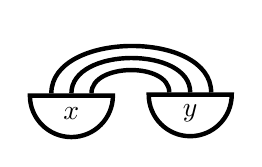
\begin{tikzpicture}[baseline, ultra thick]
    \node[draw, shape=semicircle, shape border rotate=180, minimum size=1.5em] (x) {$x$};
    \node[draw, shape=semicircle, shape border rotate=180, minimum size=1.5em, right=0.5cm of x] (y) {$y$};
    \draw (x.90) to[in=90, out=90] (y.90);
    \draw (x.135) to[in=90, out=90] (y.45);
    \draw (x.45) to[in=90, out=90] (y.135);
  \end{tikzpicture}
\]
and for many (conjecturally all) closed diagrams diagrams in $\V_0$ we can use
the relations
to evaluate to a rational function in \(\QQ(v,w)\). Of course, our basis is
far from orthonormal with respect to this pairing!

We first look at the braided bases described above, and find that, up to $n=6$, we can evaluate all matrix entries of $M_n =
\left(\langle e_i, e_j \rangle\right)_{i,j}$. We can then calculate the
determinants of these matrices, obtaining
%% These are calculated in determinants-of-inner-products.nb
\begin{align*}
\det M_3 & = - \frac{
	           \{2\} [\lambda + 5] [\lambda - 6]
             }{
               [\lambda] [\lambda - 1]
             } \\
% -((brk[0, 1] brk[0, 4]^5 brk[0, 5]^3 brk[0, 6]^4 brk[1, -6]^5 brk[
%       1, -4]^2 brk[1, -3] brk[1, 2] brk[1, 3]^2 brk[1, 5]^5 brk[
%       3, -6] brk[3, 3])/(brk[0, 2]^7 brk[0, 3]^4 brk[1, -2] brk[
%       1, -1]^8 brk[1, 0]^8 brk[1, 1] brk[2, -6] brk[2, 4]))
\det M_4 & = \frac{
              [1] [4]^5 [5]^3 [6]^4 [\lambda - 6]^5 [\lambda - 4]^2 [\lambda - 3] [\lambda + 2]
              [\lambda + 3]^2 [\lambda + 5]^5 [3\lambda - 6] [3\lambda + 3]
             }{
              [2]^7 [3]^4 [\lambda - 2] [\lambda - 1]^8 [\lambda]^8 [\lambda + 1]
              [2 \lambda - 6] [2\lambda + 4]
             } \\
% -((brk[0, 1]^7 brk[0, 4]^16 brk[0, 5]^13 brk[0, 6]^20 brk[
%       1, -6]^16 brk[1, -4]^10 brk[1, -3]^12 brk[1, 2]^12 brk[1, 
%       3]^10 brk[1, 5]^16 brk[3, -6]^6 brk[3, 3]^6 brk[4, -6] brk[4, 
%       2])/(v^2 brk[0, 2]^24 brk[0, 3]^32 brk[1, -2]^6 brk[
%       1, -1]^26 brk[1, 0]^26 brk[1, 1]^6 brk[2, -6]^12 brk[2, -3] brk[
%       2, 1] brk[2, 4]^12))
\det M_5 & = 
             \frac{
              [1]^7 [4]^{16} [5]^{13} [6]^{20} [\lambda - 6]^{16} [\lambda - 4]^{10} 
              [\lambda - 3]^{12} [\lambda + 2]^{12}
              [\lambda + 3]^{10} [\lambda + 5]^{16} [3\lambda - 6]^6 [3\lambda + 3]^6
              [4 \lambda - 6] [4\lambda + 2]
             }{
              v^2 [2]^{24} [3]^{32} [\lambda - 2]^{6} [\lambda - 1]^{26} [\lambda]^{26} [\lambda + 1]^6
              [2 \lambda - 6]^{12} [2\lambda - 3] [2\lambda + 1] [2\lambda + 4]^{12}
             } \\
\det M_6 & = \frac{
              -v^{12} [1]^{67} [4]^{80} [5]^{75} [6]^{165} [\lambda - 6]^{80} [\lambda - 5]^{15} [\lambda - 4]^{65} [\lambda - 3]^{112} [\lambda + 3]^{65} [\lambda + 4]^{15} [\lambda + 5]^{80} [2 \lambda - 4]^5 [2\lambda + 2]^5 [3\lambda - 6]^{45} [3\lambda + 3]^{45} [4 \lambda - 6]^{10} [4\lambda + 2]^{10} [5\lambda - 6] [5\lambda + 1]
             }{
               [2]^{151} [3]^{268} [\lambda - 2]^{50} [\lambda - 1]^{150} [\lambda]^{150} [\lambda + 1]^{50} [2\lambda - 6]^{107} [2\lambda - 3]^{10} [2\lambda + 1]^{10} [2\lambda + 4]^{107}
             }.
\end{align*}



In particular, we see that $\det M_4$ vanishes when $v^k = 1$ for
$k=1,2,4,5,8,10$, or $12$, or when $w = \pm v^k$ for $k=-5,-3,4,6$, or when
$v^4 \pm v^2 w + w^2 = 0$ (equivalently, $w = \zeta v^{-1}$ for $\zeta$ a
primitive 3rd or 6th root of unity) or $1 \pm v w + v^2 w^2 = 0$
(equivalently, $w = \zeta v^2$ for $\zeta$ a primitive 3rd or 6th root of
unity). Then, $\det M_5$ vanishes at all the same places, and additionally at
$v^6 + w^4 = 0$ and $1 + v^2 w^4 = 0$. \nn{These are exactly the curves
corresponding for quantum $E_6$.} Finally $\det M_6$ vanishes everywhere $\det
M_5$ does, and also at $w = \pm v^k$ for $k=-4,-2,3,5$, $w = \pm i v^k$ for
$k=-1,2$, $v = \pm w^{-5}$ and $w^5 \pm v^6 = 0$.

In fact, the components of $\det M_4 = 0$ are explained by smaller categories
which we already know about, or degenerate cases. \nn{appropriate reference
elsewhere in the paper for the $v^k = 1$ cases} At $w = \pm v^{-5}$ and $w =
\pm v^6$, we see that $d=0$, so any quotient would be degenerate. At $w = \pm
v^{-3}$ and $w = \pm v^4$, we recover the $SO(3)_q$ categories \nn{details?}.
At $w = \zeta v^2$, with $\zeta$ a primitive 3rd or 6th root, we obtain
$(G_2)_q$ \nn{details}. \nn{What about $w = \zeta v^{-1}$?}

Although it may appear that new factors are appearing in the
denominators as we look at $\det M_3, \det M_4, \det M_5, $ and $\det
M_6$, one should recall that the bracket polynomials $[a \lambda + b]$
are not generally irreducible. \nn{Does ``irreducible'' make sense?
  $\QQ[v^{\pm 1}, w^{\pm 1}]$ is not a UFD, right?} The
irreducible factors appearing in the denominator after cancellation
remain the denominators \nn{already} introduced: $\det M_4$ has poles
at $w=\pm1, v=\pm w, v^6+w^2 = 0$, and $1+v^4w^2 = 0$,
then $\det M_5$ has additional poles at $w=0, 1\pm v + v^2 = 0$, and $\det M_6$
has another pole at $v = \pm 1$.


\subsection{Matrices for operations}
In this section, we obtain matrices for the braiding and rotation operators on
 $\V_n$, `relative to' $\cB^{\text{braided}}$ described above.
We have to be careful here, as we don't know that $\cB^{\text{braided}}$
actually spans $\V_n$, or even that the braiding and rotation operators map
the span of $\cB^{\text{braided}}$ to itself.

The second of these questions is relatively tractable; it would just be a
matter of applying a braiding or rotation to each element, and showing that it
is possible to use the relations to rewrite the result as a linear combination
of elements of $\cV^{\text{braided}}$. We take a slightly different approach,
computing the matrix which \emph{would} be associated to each of the
operations \emph{if} $\cB^{\text{braided}}$ really were a basis, and then
verifying that these matrices satisfy the expected properties.


Now, given an operator $T: \V_n \to \V_m$, if the $\cB^{\text{braided}}_n$
are bases, the associated matrix for $T$ would be $AM_m^{-1}$, where
$A = \left(\langle T e_i, e_j \rangle\right)_{i,j}$.
Rather unfortunately inverting the matrix $M_6$ is computationally
infeasible. (Recall that arithmetic over $\QQ(v,w)$ may be quite inefficient!)

We find, nevertheless, that for $T$ any of 
\begin{align*}
  (\rho_n : \V_n \to \V_n) & = 
    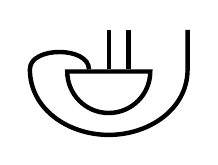
\begin{tikzpicture}[baseline, ultra thick]
      \node[draw, shape=semicircle, shape border rotate=180, minimum size=1.5em] (x) {};
      \draw (x.90) -- ++(0,0.5);
      \draw (x.45) -- ++(0,0.5);
      \draw (x.135) to[in=90, out=90] ++(-0.75,0) 
                     to[in=180,out=-90] ($(x.-90)+(0,-0.25)$) 
                     to[out=0,in=-90] ($(x.45)+(0.75,0)$)
                     -- ++(0,0.5);
    \end{tikzpicture} &
  (\beta_n : \V_n \to \V_n) & = 
    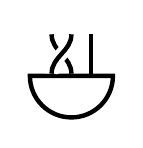
\begin{tikzpicture}[baseline, ultra thick]
      \node[draw, shape=semicircle, shape border rotate=180, minimum size=1.5em] (x) {};
      \draw (x.45) -- ++(0,0.5);
      \draw (x.90) to[out=90,in=-90] ($(x.135)+(0,0.5)$);
      \draw[knot] (x.135) to[out=90,in=-90] ($(x.90)+(0,0.5)$);
    \end{tikzpicture} 
  \displaybreak[1] \\
  (\cap_n : \V_n \to \V_{n-2}) & = 
    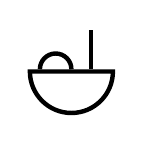
\begin{tikzpicture}[baseline, ultra thick]
      \node[draw, shape=semicircle, shape border rotate=180, minimum size=1.5em] (x) {};
      \draw (x.45) -- ++(0,0.5);
      \draw (x.90) arc (0:180:0.2);
    \end{tikzpicture}
  &
  (\cup_{n-2} : \V_{n-2} \to \V_{n}) & = 
    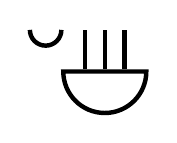
\begin{tikzpicture}[baseline, ultra thick]
      \node[draw, shape=semicircle, shape border rotate=180, minimum size=1.5em] (x) {};
      \draw (x.90) -- ++(0,0.5);
      \draw (x.45) -- ++(0,0.5);
      \draw (x.135) -- ++(0,0.5);
      \draw ($(x.135)+(0,0.5)+(-0.3,0)$) arc (0:-180:0.2);
    \end{tikzpicture}
  \displaybreak[1] \\
  (\fork_{n-1} : \V_{n-1} \to \V_{n}) & = 
    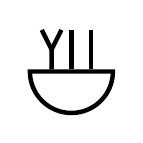
\begin{tikzpicture}[baseline, ultra thick]
      \node[draw, shape=semicircle, shape border rotate=180, minimum size=1.5em] (x) {};
      \draw (x.90) -- ++(0,0.5);
      \draw (x.45) -- ++(0,0.5);
      \draw (x.135) -- ++(0,0.25) -- ++(0.125,0.25);
      \draw    ($(x.135)+(0,0.25)$) -- ++(-0.125,0.25);
    \end{tikzpicture}
  &
  (\fuse_n : \V_n \to \V_{n-1}) & = 
    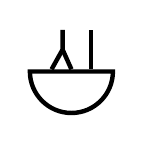
\begin{tikzpicture}[baseline, ultra thick]
      \node[draw, shape=semicircle, shape border rotate=180, minimum size=1.5em] (x) {};
      \draw (x.45) -- ++(0,0.5);
      \draw (x.90) -- ($(x.114)+(0,0.25)$);
      \draw (x.135) -- ($(x.114)+(0,0.25)$) -- ++(0,0.25);
    \end{tikzpicture}
  \\
  (H_n : \V_n \to \V_n) & = 
    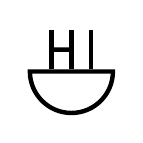
\begin{tikzpicture}[baseline, ultra thick]
      \node[draw, shape=semicircle, shape border rotate=180, minimum size=1.5em] (x) {};
      \draw (x.45) -- ++(0,0.5);
      \draw (x.90) -- ++(0,0.5);
      \draw (x.135) -- ++(0,0.5);
      \draw ($(x.90)+(0,0.25)$) -- ($(x.135)+(0,0.25)$);
    \end{tikzpicture}
\end{align*}
with $n \leq 6$,
we can evaluate all of the matrix entries of $A$ as rational functions.
(Even though $H_n = \rho_{n}^{-1} \fuse_n \rho_{n+1} \fork_n$, we can not
use this to compute $H_6$ as we would need to know $\rho_7$ and $\fuse_7$.)

Even though directly inverting $M$ is infeasible, we find that we can
calculate the product $A M^{-1}$ in each case. (Nevertheless this remains a
difficult calculation ---  we use some tricks, calculating the product at
various specialisations of the variables and then using interpolation, finally
verifying our answer by multiplying by $M$.)

Explicit matrices are available with the {\tt arXiv} sources of this article, 
as the files $$\text{{\small\tt matrices/n-box-OP-matrix.m}},$$ where $n \leq 6$, and {\tt OP}
is one of {\tt rotation},
{\tt braiding}, {\tt inverse-braiding}, {\tt cup}, {\tt cap}, {\tt fork}, {\tt
fuse}, {\tt H}. 
The matrices are written in terms of the variables $d, v$. 


\subsection{Representations of braid groups}
The affine $n$-strand braid group has generators $\rho$ and $\beta$, with
relations $\rho^n = 1$, $\beta \rho^\pm \beta \rho^\mp \beta = \rho^\pm
\beta \rho^\mp \beta \rho^\pm
\beta \rho^\mp$, and $\beta \rho^i \beta \rho^{-i} = \rho^i \beta \rho^
{-i} \beta$ for all $i = 2, \ldots, n-2$.

At this point, we may verify that the matrices $\rho = \rho_n$ and $\beta =
\beta_n$ provide a representation of the affine $n$-strand braid group merely by multiplying out the matrices. 

\begin{lemma}
The matrices described in the previous section give a representation of the affine $n$-strand braid group for $3 \leq n \leq 6$.
\end{lemma}


\subsection{A 2-variable link polynomial}

\subsubsection{Limited planar operations}
Thinking of the vector spaces $\V_n$ as forming a planar algebra, 
at this point we have limited access to the full set of operations indexed by
planar tangles. We have computed above
$\cap_n : \V_n \to \V_{n-2}$, 
$\cup_{n-2} : \V_{n-2} \to V_n$, and
$\rho_n: \V_n \to \V_n$ for $n \leq 6$. We can also find
\begin{align*}
(m_{4,4,2} : \V_4 \otimes \V_4 \to \V_4) & = 
  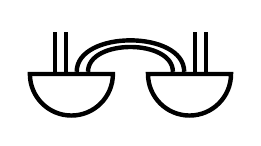
\begin{tikzpicture}[baseline, ultra thick]
    \node[draw, shape=semicircle, shape border rotate=180, minimum size=1.5em] (x) at (0,0) {};
    \node[draw, shape=semicircle, shape border rotate=180, minimum size=1.5em] (y) at (1.5,0) {};
    \draw (x.130) -- +(0,0.5);
    \draw (x.105) -- +(0,0.5);
    \draw (x.75) to[out=90,in=90] (y.105);
    \draw (x.50) to[out=90,in=90] (y.130);
    \draw (y.75) -- +(0,0.5);
    \draw (y.50) -- +(0,0.5);
  \end{tikzpicture}
 \displaybreak[1] \\
(m_{4,6,2} : \V_4 \otimes \V_6 \to \V_6) & = 
  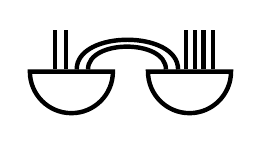
\begin{tikzpicture}[baseline, ultra thick]
    \node[draw, shape=semicircle, shape border rotate=180, minimum size=1.5em] (x) at (0,0) {};
    \node[draw, shape=semicircle, shape border rotate=180, minimum size=1.5em] (y) at (1.5,0) {};
    \draw (x.130) -- +(0,0.5);
    \draw (x.105) -- +(0,0.5);
    \draw (x.75) to[out=90,in=90] (y.120);
    \draw (x.50) to[out=90,in=90] (y.140);
    \draw (y.100) -- +(0,0.5);
    \draw (y.75) -- +(0,0.5);
    \draw (y.55) -- +(0,0.5);
    \draw (y.40) -- +(0,0.5);
  \end{tikzpicture}
 \displaybreak[1] \\
\intertext{and}
(m_{4,4,1} : \V_4 \otimes \V_4 \to \V_6) & = 
  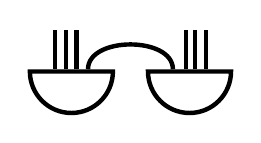
\begin{tikzpicture}[baseline, ultra thick]
    \node[draw, shape=semicircle, shape border rotate=180, minimum size=1.5em] (x) at (0,0) {};
    \node[draw, shape=semicircle, shape border rotate=180, minimum size=1.5em] (y) at (1.5,0) {};
    \draw (x.130) -- +(0,0.5);
    \draw (x.105) -- +(0,0.5);
    \draw (x.75) -- +(0,0.5);
    \draw (x.50) to[out=90,in=90] (y.130);
    \draw (y.100) -- +(0,0.5);
    \draw (y.75) -- +(0,0.5);
    \draw (y.50) -- +(0,0.5);
  \end{tikzpicture}
\end{align*}
 as follows.

Recall that our chosen basis for $\V_4$ is
\[
  \left(
    \tikz[baseline=-7, ultra thick]{\draw(0,0) arc (-180:0:0.2); \draw(0.6,0) arc(-180:0:0.2);},
    \tikz[baseline=-7, ultra thick]{\draw(0,0) arc (-180:0:0.4); \draw(0.2,0) arc(-180:0:0.2);},
    \tikz[baseline=-7, ultra thick]{\draw(0,0) arc (-180:0:0.2); \draw(0.6,0) arc(-180:0:0.2);
                       \draw(0.2,-0.2) arc (-180:0:0.3);},
    \tikz[baseline=-7, ultra thick]{\draw(0,0) arc (-180:0:0.4); \draw(0.2,0) arc(-180:0:0.2);
                       \draw(0.4,-0.4) -- (0.4,-0.2);},
    \tikz[baseline=-7, ultra thick]{\draw(0,0) arc (-180:0:0.3); \draw[knot] (0.3,0) arc (-180:0:0.3);}
  \right)
\]
Expressed in our chosen bases, we then have 
\begin{align*}
  m_{4,n,2}((x_1, x_2, x_3, x_4, x_5) \otimes y)
    & = x_1 \cup_{n-2}\cap_n y \\
      & \quad + x_2 y \\
      & \quad + x_3 \fork_{n-1}\fuse_n y \\
      & \quad + x_4 H_n y \\
      & \quad + x_5 \beta y.
\end{align*}
Finally, we can write $m_{4,4,1}$ in terms of the other operations, e.g.
as
$$
 m_{4,4,1}(x \otimes y) = m_{4,6,2}(x \otimes \rho_6^{-1} (\cup_4 (\rho_4(y)))
 = 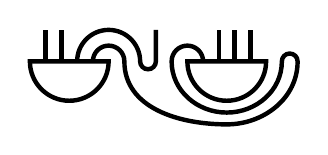
\begin{tikzpicture}[baseline, ultra thick]
     \draw (0,0) arc (-180:0:0.5) -- cycle;
     \draw (2,0) arc (-180:0:0.5) -- cycle;
     \draw (2.2,0) arc (0:180:0.2) to[out=-90,in=180] (2.5,-0.65) to[out=0,in=-90] (3.2,0) arc (180:0:0.1) to[out=-90,in=0] (2.5,-0.8) to[out=180,in=-90] (1.2,0) arc (0:180:0.2);
     \draw (0.6,0) arc (180:0:0.4) arc (-180:0:0.1) -- +(0,0.4);
     \draw (0.2,0) -- +(0,0.4);
     \draw (0.4,0) -- +(0,0.4);
     \draw (2.4,0) -- +(0,0.4);
     \draw (2.6,0) -- +(0,0.4);
     \draw (2.8,0) -- +(0,0.4);
   \end{tikzpicture}
$$ 

\subsubsection{Conway girth}
Typically, we may choose to think about a diagrammatically defined tangle 
invariant as a morphism of planar algebras 
$\mathsf{Tangle} \to \mathcal{Q}$ for some planar algebra
$\mathcal{Q}$, sending the crossing to a suitable element of $\mathcal{Q}_4$.
\nn{$\mathsf{Tangle}$ has not been defined.}
In our case we only know a limited set of operations in the target planar
algebra, and so can only compute the invariants of links which we can generate
from the crossing using those available planar operations.

\begin{definition}
The \emph{width} of a planar graph generically embedded in the plane is the 
maximum number of intersections with a horizontal line. The width of a planar
graph is the minimum width over all generic embeddings.

The \emph{Conway width} of a 4-valent planar graph is the width of the graph 
after repeatedly collapsing all digons. The Conway width of a link is the
Conway width of its shadow.
\end{definition}

It is easy to see that with the available planar operations, we can evaluate 
all Conway width 6 links.

\begin{lemma}
All knots and links with at most 12 crossings with the two exceptions
$$
\diagram{0.2}{a6b1b1be704dda48723477a9c4e57cf27a610f7c} \qquad
\diagram{0.2}{d152a4e30d0711d71caa5a012365e5adbdcd5b2c}
$$
%% How did I generate these graphs?! I guess with DrawPlanarGraphApp.scala, setting `withOutputPath' appropriately?
% 12C = cuboctahedron
% a6b1b1be704dda48723477a9c4e57cf27a610f7c
% PlanarGraph(35,Vector(List(), List((5,6), (4,9), (3,8), (2,7)), List((2,6), (10,7), (9,18), (8,17)), List((8,6), (15,17), (14,27), (13,26)), List((10,18), (3,7), (19,8), (18,35)), List((18,18), (26,35), (25,46), (24,45)), List((24,18), (31,45), (15,27), (9,17)), List((26,46), (19,35), (35,8), (34,54)), List((34,46), (42,54), (41,65), (40,64)), List((40,46), (47,64), (31,27), (25,45)), List((42,65), (35,54), (4,8), (50,9)), List((50,65), (5,9), (13,6), (56,26)), List((56,65), (14,26), (47,27), (41,64))),Vector((2,0), (2,0), (2,0), (2,0), (2,0), (2,0), (2,0), (2,0), (2,0), (2,0), (2,0), (2,0)),0)
% 12G
% d152a4e30d0711d71caa5a012365e5adbdcd5b2c
% PlanarGraph(46,Vector(List(), List((5,6), (4,9), (3,8), (2,7)), List((2,6), (10,7), (9,18), (8,17)), List((8,6), (15,17), (14,27), (13,26)), List((13,6), (20,26), (19,36), (5,9)), List((26,36), (25,46), (24,45), (19,9)), List((20,36), (14,26), (30,27), (26,46)), List((10,18), (3,7), (34,8), (33,54)), List((4,8), (24,9), (40,45), (34,54)), List((25,45), (47,46), (46,75), (40,54)), List((54,75), (53,86), (33,18), (46,54)), List((15,27), (9,17), (53,18), (57,86)), List((47,75), (30,46), (57,27), (54,86))),Vector((2,0), (2,0), (2,0), (2,0), (2,0), (2,0), (2,0), (2,0), (2,0), (2,0), (2,0), (2,0)),0)
have Conway width at most 6.
\end{lemma}
\begin{proof}
The Conway width of a link is the width of the Conway basic polyhedron 
obtained after collapsing all digons. One can enumerate the basic polyhedron
with $n$ vertices using Brinkmann and McKay's {\tt plantri} program
\cite{MR2357364,MR2186681}, with the command {\tt plantri -qda -c2 <n+2>}. 
All basic polyhedra with less than 12 vertices have width at most 6, and of 
the 12 vertex basic polyhedra all but 12C (the cuboctahedron) and 12G (using 
the naming scheme from \cite{MR679310}) have width at most 6. These graphs,
made into alternating links, are the two exceptions described above.
\nn{Say something about non-alternating versions of these links}
\end{proof}
In fact, almost all prime knots up to 11 crossings have bridge number 
at most 3, and hence width at most 6, with 15 exceptions, all Montesinos
knots. \footnote{The exceptions are 11a43, 11a44, 11a47, 11a57, 11a231,
  11a263, 11n71, 11n72, 11n73, 11n74, 11n75, 11n76, 11n77, 11n78, and
  11n81. \cite{1208.4233}}
Montesinos knots are easily seen to have Conway width 4.
Interestingly all knots with at most 14 crossings have Conway width at most 6.
If we were able to work with Conway width 8, we could nearly exhaust the 
available tables of knots and links; every Conway basic polyhedron with at 
most 19 vertices has width at most 8.

The obvious greedy algorithm (repeatedly collapse digons, when that is not 
possible apply $m_{4,4,1}$ to merge two 4-boxes into a 6-box, and afterwards
hope that $m_{6,4,2}$  suffices to combine all remaining 4-boxes into that
6-box) works on all but one prime knot up to 12 crossings, except \nn{... is
it worth explaining this? perhaps it illustrates the greedy algorithm}

\subsubsection{Examples}
Using the above observations, we have computed the (conjectural!) 
invariant $\xi$ of all prime links up to 11 crossings, and all prime knots up
to 12 crossings. We observe that the values of $\xi$ are always of the form
$$\xi(L) - d^{k} = 
\frac{[3][4][\lambda-6][\lambda+5]}{[1][2][\lambda-1]^{k+1} [\lambda]^{k+1}} \mathcal E(L),$$
where $d = \xi(\textrm{unknot}) = ...$, $k$ is the number of components of $L$, 
and $\mathcal E(L)$ is some Laurent polynomial (not just a rational function)
in $v$ and $w$. These polynomials $\mathcal E (L)$ are tabulated
\nn{ at ...}, and in machine readable format as \nn{...} in the {\tt arXiv} sources.

It would be desirable to verify that these computed invariants specialize 
correctly to the quantum link invariants of the adjoint representations of the
exceptional Lie algebras.
\DPTtodo{Don't we have an unconditional theorem here, that these do in fact
  specialize correctly?}
Unfortunately, these invariants have previously been
rather hard to compute, so there is little available to check against. The Lie
algebra $\mathfrak{sl}_2$ lies on the exceptional curve, and so the 2nd
coloured Jones polynomial  (that is, colored by the 3-dimensional adjoint
representation) should be the \nn{$w = ...,  v= ...$} specialisation. This is
indeed the case for all the links tabulated above.

Even for the adjoint representation of $G_2$, an earlier program by the first
author for computing quantum knot invariants gets only as far as the trefoil. 
Sure enough, we have
$$\xi(3_1) = ...$$
which at \nn{$w = ...,  v= ...$} gives \nn{...}

\nn{check using the adjoint representation skein theory provided by Greg; many errors in his formulas!}

The fact that $\xi(12^n_{...}) = ...$ suggests that the $E_8$ adjoint quantum 
knot invariant should be $$...$$, but previous methods haven't come close to
computing this.

\subsubsection{Knotted trivalent graphs}\mbox{}%
\nn{just some examples}
\nn{including the unknotted dodecahedron}

\subsubsection{Comparisons}
\nn{Compare to Westbury and the other paper...}


\section{When $v$ is a small root of unity}

The goal of this section is to analyze what happens when $v$ is a $10$th or $12$th root of unity, so that the derivation of the QESquare and QECrossing relations break down.  We begin by analyzing what happens when $\dim \cC_4 < 5.$


\subsection{Corner cases with small $4$-box space}

\begin{lemma}
The diagrams
$$\cupcap \text{ and } \twostrandid$$
are non-zero and are linearly independent.
\end{lemma}
\begin{proof}
If either diagram is zero then by multiplying by a crossing on the appropriate side you get that the trivalent vertex is zero, which is a contradiction.  If the two diagrams are linearly dependent, then again multiplying by a trivalent vertex would show that the trivalent vertex is zero.
\end{proof}


The following lemma is a mild generalization of \cite{???} where we have relaxed the non-degeneracy assumption.


\begin{lemma}
Suppose that the diagrams   
  \[
  \cupcap\;,\qquad\twostrandid\;,
    \qquad\drawI\;,\qquad\drawH\;\;
   \]
are linearly dependent, then
 
$$\drawI\; - \; \drawH - \frac{1}{d-1} \left(\twostrandid - \cupcap \right) = 0.$$
\end{lemma}
\begin{proof}
If the two Temperley-Lieb diagrams are linearly dependent, then attaching a trivialent vertex shows that the trivalent vertex is zero which is a contradiction.  So we must have a relation of the form:
$$\drawI\;\pm \; \drawH = z \left(\twostrandid \pm \cupcap \right).$$

Capping off we see that $b= z (d \pm 1)$, so $z = \frac{b}{d \pm 1}$.  So all we need to do is exclude the $+$-sign case.

Attaching a trivalent vertex we see that $t + b = \frac{b}{d + 1}$, so $t =  -\frac{b d}{d + 1}$.  Adding $\drawH$ to the top gives:

$$t \drawI + \ngon[45]{4} = \frac{b}{d+1} \left( \drawH + b \cupcap\right).$$

If we take this relation minus its $90$-degree rotation the square term will vanish yielding:
$$ b \frac{d-1}{d+1} \left( \drawI -\drawH \right) = \frac{b^2}{d+1} \left(\twostrandid - \cupcap\right).$$
Dividing by $b \frac{d-1}{d+1}$ yields the desired equation.
\end{proof}

By Lemma \ref{lem:IequalsH} we have the following Corollary.

\begin{corollary}
If the diagrams   
  \[
  \cupcap\;,\qquad\twostrandid\;,
    \qquad\drawI\;,\qquad\drawH\;\;
   \]
are linearly dependent, then
\begin{itemize}
\item $v$ is a primitive $12$th root of unity
\item $\cC$ is a quotient of $SO(3)_q$ with the usual braiding
\item $\cC$ is $\mathrm{Rep}(S_3)$ with its symmetric braiding.
\end{itemize}
\end{corollary}


\begin{proposition} \label{prop:dim4}
If the diagrams  
  \[
  \cupcap\;,\qquad\twostrandid\;,
    \qquad\drawI\;,\qquad\drawH\;,\qquad\braidcross\;,\qquad\ngon[45]{4}\;
   \]
span a space of dimension $4$ or smaller, then
\begin{itemize}
\item $v$ is a primitive $12$th root of unity
\item $\cC$ is a quotient of $SO(3)_q$ with the usual braiding.
\item $\cC$ is $\mathrm{Rep}(S_3)$ with its symmetric braiding.
\item $\cC$ is a quotient of $(G_2)_q$ with the usual braiding.  \NStodo{Which QEJacobi hold?}
\end{itemize}
\end{proposition}
\begin{proof}
If the first four diagrams are linearly dependent then we're in one of the first three cases.  Otherwise, we have a relation simplifying both the crossing and the square in terms of the first four diagrams.  This means that $\cC$ is generated by the trivalent vertex and $\dim \cC_4 \leq 4$, thus by a modification of \cite{???} we see that $\cC$ is a quotient of $(G_2)_q$.
\end{proof}

\begin{remark}
Strictly speaking in \cite{???} we only considered non-degenerate trivalent categories, but this can be avoided as follows.  The argument that the pentagon reduces still applies, so all small faces reduce, and non-elliptic diagrams span all $\cC_k$.  If the $10$ non-elliptic diagrams in $\cC_5$ are independent then Kuperberg\cite{???} says that $\cC$ is a quotient of $(G_2)_q$.  If there's a relation between these ten diagrams, the relation must be negligble.  By \cite{???} either there's a single relation and the category is a quotient of $(G_2)_{\zeta_{10}}$, or the non-degenerate quotient of $\cC$ is an $ABA$ category which contradicts $\cC$ being braided.
\end{remark}



\subsection{The case $v = \pm 1$}

Throughout this section we assume $v=1$.

Recall $t = \frac{b-[5]\alpha}{\{2\}} = \frac{b}{2}$.  We also have that $0= [5]b = -\alpha (d+\{8\})$, so we split into two cases based on whether $\alpha = 0$.

\begin{lemma}
There are no $\cC$ with $\alpha \neq 0$.
\end{lemma}
\begin{proof}
Since $d+\{8\}=0$, we have that $d=-2$.  The QECrossing relation says that:
$$\braidcross + \cupcap + \twostrandid = 0.$$
This is exactly the case excluded in Lemma \ref{lem:betazero}.
\end{proof}

\begin{lemma}
If $\alpha = 0$, then $\cC$ satisfies the defining relations of the classical exceptional series.
\end{lemma}
\begin{proof}
QECrossing says that the crossing is symmetric, and then QEJacobi becomes the usual Jacobi relation. 

Since $\dim \cC_4 \leq 5$, there must be some relation of the following form:
$$0 = \ngon[45]{4} + x \symcross + y \left(\drawI + \drawH \right) + z\left(\twostrandid + \cupcap \right).$$
Multiplying this by a crossing and using the Jacobi relation:
\begin{align*}
0 &= \ngon[45]{4} - \frac{b}{2} \drawI + x \twostrandid + y \left(-\drawI + \drawH -\drawI \right) + z\left(\symcross + \cupcap \right) 
\\ &= \ngon[45]{4} + z \symcross + \left(-2y -\frac{b}{2} \right) \drawI +y \drawH +x \twostrandid + z\cupcap. 
\end{align*}

If these two relations are distinct, then Proposition \ref{prop:dim4} applies, and the only case with $v=1$ is classical $SO(3)$ (note that there is not trivalent category $(G_2)_{\zeta_3}$), which satisfies the classical exceptional relation.  Otherwise, we have $x=z$ and $y = -\frac{b}{6}$.  

Capping off this relation gives $0 = b^2 + x -\frac{b^2}{6}+x(1+d) =  (2+d)x +\frac{5 b^2}{6}$, so we have $x = -\frac{5 b^2}{6(2+d)}$.  This gives the classical exceptional square relation.
\end{proof}


\subsection{The case $v$ is a primitive third or sixth root of unity}

\begin{proposition}
If $v$ is a primitive third root of unity, then $\cC$ is classical $SO(3)$ or classical $G_2$.
\end{proposition}
\begin{proof}
Since $v$ is not a $10$th root of unity $\alpha$ is non-zero.  Also $b+[3]\alpha = b \neq 0$.  QECrossing says that the braiding is symmetric.  
%QEJacobi becomes $$\drawsymcrossX + v \drawI - v^2 \drawH + \alpha \left(\symcross + v^2 \twostrandid +v \cupcap \right) = 0.$$

QESquare becomes:
$$\symcross+\frac{\sqrt{-3}}{2\alpha} \left(\drawI + \drawH \right) -\frac{1}{2} \left(\twostrandid + \cupcap \right) = 0.$$

After rescaling the trivalent vertex, this becomes precisely the Hurwitz relation (or classical $G_2$ relation) of \cite{???}.  The main result of that paper is that either $d = 7$ and $\cC$ is classical $G_2$ or $d=3$ and $\cC$ is $SO(3)$.
\end{proof}

\subsection{The case $v$ is a primitive fourth root of unity}

Since $v$ is not a $10$th root of unity $\alpha$ is nonzero.  We have that $d+2 = \frac{-2ib}{\alpha}$.
We need to split into two cases based on whether $b+[3]\alpha = 0$.  

\begin{proposition}
If $b+[3]\alpha \neq 0$ then $\cC$ satisfies the relations of the classical F4 relation.  In particular the non-degenerate quotient of $\cC$ must be one of LIST.
\end{proposition}
\begin{proof}
If $b+[3]\alpha \neq 0$, then QECrossing says the crossing is symmetric.   QEJacobi becomes
$$\drawsymcrossX + \drawI + \drawH = \alpha i \left(\symcross + \twostrandid + \cupcap \right).$$  If we rescale the trivalent vertex so that $\alpha i = 2$ then $b = d+2$ we have exactly the classical F4 relation.  The main result of \cite{???} is that this forces one of the following possibilities:

TABLE

We exclude the $\Rep(S_3)$ case because it satisfied $b+[3]\alpha = 0$.
\end{proof}

Since we do not know whether the classical F4 relation is sufficient for evaluating all closed diagrams, we do not know whether there are any additional degenerate $\cC$ whose non-degenerate quotient is one of the above categories.

If $b+[3]\alpha = 0$, then $\alpha = -\frac{bi}{2}$ and $d = 2$.  QEJacobi becomes
$$\drawcrossX + \drawI + \drawH = \frac{1}{2} \left(\braidcross + \twostrandid + \cupcap \right).$$
QESquare becomes
$$\ngon[45]{4} = -\frac{1}{2} \left(\drawI + \drawH \right) + \frac{1}{2} \left(\twostrandid + \cupcap\right).$$

\begin{lemma}
The following diagrams are negligible in $\cC$:
\begin{itemize}
\item $$\braidcross + \invbraidcross - 2 \left(\drawI + \drawH \right)$$
\item $$\braidcross - \invbraidcross$$
\item $$\left(\drawI - \drawH - \twostrandid + \cupcap\right).$$
\end{itemize}
\end{lemma}
\begin{proof}
If the diagrams
  \[
  \cupcap\;,\qquad\twostrandid\;,
    \qquad\drawI\;,\qquad\drawH\;,\qquad\braidcross\;\qquad\ngon[45]{4}\;
   \]
 span a $4$-dimensional space then the first $4$ diagrams span by Proposition \ref{prop:dim4}\NStodo{Add this statement to Prop \ref{prop:dim4}}.  If these $5$ diagrams are linearly independent then since $\dim \cC_4 \leq 5$, then they span.  Thus in either case we can check whether an element is negligible by pairing it with the above $5$ diagrams.
\end{proof}

\begin{corollary}
If $\cC$ is non-degenerate then it must be $\mathrm{Rep}(S_3)$.
\end{corollary}

\begin{corollary}
Either
\begin{itemize}
\item $$\braidcross + \invbraidcross = 2 \left(\drawI + \drawH \right).$$
\item $$\braidcross - \invbraidcross = x \left(\drawI - \drawH - \twostrandid + \cupcap\right).$$
\end{itemize}
\end{corollary}

If both relations hold, then the crossing simplifies.  By \ref{prop:dim4}, we see that $\cC$ is $\mathrm{Rep}(S_3)$ (which satisfies the latter relation for all $x$) or $(G_2)_{\zeta_{12}}$ for some primitive $12$th root of unity (which satisfies the latter relation for $x = \pm \frac{2}{\sqrt{-3}}$). Note that for each value of $v$ there are two distinct such $(G_2)_{\zeta_{12}}$ as ribbon categories, but they're equivalent as pivotal categories.
\NStodo{Check sign, and find relationship between $\zeta$ and $v$}

\begin{conjecture}
Trivalent ribbon graphs modulo $d=2$ and the following relations:
$$\drawcrossX + \drawI + \drawH = \frac{1}{2} \left(\braidcross + \twostrandid + \cupcap \right)$$
$$\ngon[45]{4} = -\frac{1}{2} \left(\drawI + \drawH \right) + \frac{1}{2} \left(\twostrandid + \cupcap\right)$$
$$\braidcross + \invbraidcross = 2 \left(\drawI + \drawH \right)$$

gives a category $\cG$ with finite dimensional Hom-spaces and $\dim \cG_k = 1,0,1,1,5$ for $k = 0,1,2,3,4$.  
\end{conjecture}

Note that these generators and relations can't define a trivial category because it has a quotient to  $(G_2)_{\zeta_12}$, and they also can't define can't define $(G_2)_{\zeta_12}$ because it has braided quotient maps to both $(G_2)_{\zeta_12}$ and $(G_2)_{-\zeta_12}$.  So the content of this conjecture is that these relations suffice to simplify diagrams down to the appropriate spanning sets.

\begin{conjecture}
Trivalent ribbon graphs modulo $d=2$ and the following relations:
$$\drawcrossX + \drawI + \drawH = \frac{1}{2} \left(\braidcross + \twostrandid + \cupcap \right)$$
$$\ngon[45]{4} = -\frac{1}{2} \left(\drawI + \drawH \right) + \frac{1}{2} \left(\twostrandid + \cupcap\right)$$
$$\braidcross - \invbraidcross = \frac{2}{\sqrt{-3}} \left(\drawI - \drawH - \twostrandid + \cupcap\right).$$

gives a non-trivial category $\cH$ with $\dim \cH_k = 1,0,1,1,5$ for $k = 0,1,2,3,4$.  
\end{conjecture}

Again $\cH$ has braided quotient maps to both $(G_2)_{\zeta_12}$ and $(G_2)_{-\zeta_12}$ (which are the same as categories but not braided categories), so the content of this conjecture is that these relations suffice to simplify diagrams down to the appropriate spanning sets.

\begin{conjecture}
Trivalent ribbon graphs modulo $d=2$ and the following relations:
$$\drawcrossX + \drawI + \drawH = \frac{1}{2} \left(\braidcross + \twostrandid + \cupcap \right)$$
$$\ngon[45]{4} = -\frac{1}{2} \left(\drawI + \drawH \right) + \frac{1}{2} \left(\twostrandid + \cupcap\right)$$
$$\braidcross - \invbraidcross = 0.$$

gives a non-trivial category $\cF$ with $\dim \cF_k = 1,0,1,1,5$ for $k = 0,1,2,3,4$.
\end{conjecture}

$\cF$ is the classical F4 family at $d=2$ without taking the non-degenerate quotient.  There is some evidence given in \cite{???} that these relations are enough to simplify closed diagrams.  In this case it's possible that these relations collapse all the way down to $\mathrm{Rep}(S_3)$ with $\dim \cF_4 = 4$ or that $\dim \cF_4 = 4$.

\begin{remark}
We expect that $\cF$ has an infinitesimal deformation defined over $\mathbf{C}[\varepsilon]/\varepsilon^2$ where $d = 2+\varepsilon$ as suggested by the double root in \cite{???}.  This infinitesimal deformation should have a (non-braided) quotient to an infinitesimal deformation of $(G_2)_{\zeta_12}$.
\end{remark}

We have no idea what to expect if you impose the relation 
$$0 = \braidcross - \invbraidcross = x \left(\drawI - \drawH - \twostrandid + \cupcap\right)$$
for some $x$ that is neither $0$ nor $\pm \frac{2}{\sqrt{-3}}$.


\section{From the classical to the quantum conjecture}
\label{sec:classical-quantum}

We now show that the classical consistency conjecture implies
the quantum consistency conjecture, for suitable base
rings.
\begin{theorem}\label{thm:classical-quantum}
  If Conjecture~\ref{conj:class-consist} is true
  for $\mathrm{Exc}_{R,\lambda}$, then
  Conjecture~\ref{conj:quant-consist} is true for
  $\mathrm{QExc}_{R((h)),v,w}$ for $v=e^{h/4}$ and $w=e^{\lambda
    h/4})$ as formal Laurent series.
\end{theorem}
This section will be devoted to a proof of
Theorem~\ref{thm:classical-quantum}. Let $\eval$ be the functor from
$\mathsf{Jac}_{R,d,b}$ to $\mathsf{Exc}_{R,\lambda}$ given by hypothesis.

The first step is constructing
the conjectured functor from tangles $\Qeval$, for which the main
ingredient is the
\emph{Kontsevich integral}~$Z$. The Kontsevich integral was first
defined for unframed knots \cite{MR1318886}, and later extended to
framed trivalent graphs \cite{MR1473309,MR2304469,MR2661529}. We
briefly recall its properties. We specialize to the case corresponding
to the adjoint representation of the Lie algebra, removing the usual
distinction between the two different kinds of edges.

Let $\mathsf{TriTrangle}$ be the category of framed, unoriented,
trivalent graph tangles. \nn{Maybe this definition should be earlier.}
Then, for ring $R$ containing~$\QQ$ and $d,b \in R$, $Z$ is a functor
from $\mathsf{TriTangle}$ to
$\mathsf{Jac}_{R[[h]],d,b}$.
\nn{are we using \texttt{mathrm} or \texttt{mathsf}?}
The variable $h$ is used to keep track
of the grading. $Z$ is usually defined as a functor from the category
of parenthesized (non-associative) tangles; to define it as a functor
from our category, where the objects are just integers, for each~$n
\ge 3$, pick arbitrarily a parenthesization of $n$ objects and apply
the usual functor.

We will use the following properties of~$Z$.
\begin{enumerate}
\item\label{item:Kontsevich-perturb} $Z(G) = G + O(h)$, where on the
  right hand side we think of the
  underlying trivalent graph of~$G$ as a Jacboi diagram.
\item\label{item:Kontsevich-crossing} On a single crossing, $Z$ takes
  the value
  \begin{equation}
    \label{eq:Kontsevich-crossing}
    Z\biggl(\;\braidcross\;\biggr) =
    \exp\left(\frac{h}{2}\;\drawH\;\right)
    \cdot\; \symcross\;.
  \end{equation}
\end{enumerate}

Then the desired functor $\Qeval$ is the composition of $Z$ with the
classical evaluation $\eval$, with scalars extended to $R[[h]]$. We
then localize at $h$ to take values in the field
$\mathsf{Except}((h))$.

By hypothesis, the k-box space of $\mathsf{Except}((h))$ for $k \le 4$
have the required dimensions for a ribbon trivalent category. By
property~\eqref{item:Kontsevich-perturb} of~$Z$,
$\mathsf{Except}((h))$
is generated as a ribbon category over $R((h))$ by a
trivalent vertex.
Furthermore, Equation~\eqref{eq:Kontsevich-crossing} shows that
 that
\begin{align*}
  \Qeval\biggl(\;\twist\;\biggr) &= e^{hb/2}\eval\biggl(\;\drawcup\;\biggr)\\
  \Qeval\biggl(\;\twistvertex\;\biggr) &= e^{hb/4}\eval\biggl(\;\nvertex[-90]{3}\;\biggr)
\end{align*}
Comparison with Equation~\eqref{eq:simple-rels-spec} shows that we
should choose $v = e^{hb/24} \in R((h))$. Then by Theorem~\ref{thm:Jacobi}, the
functor $\eval$ satisfies Equation~\eqref{eq:quant-except-gen} for
some value of~$\alpha$. Note that $v^n - 1$ is
invertible for all $n \ne 1$. Thus by Lemma~\ref{lem:bplus3alpha} and
Theorem~\ref{thm:square-crossing} we renormalize~$b$ and make the
change of variables
from Equation~\eqref{eq:change-variables} to get the category
$\mathsf{QExc}_{R((h^t)),v,w}$ for some rational~$t$ and some choice
of~$w$. To identify~$w$ (and see that we can take $t=1$), 
we find the eigenvalues
of the twist operator on the 4-box space.

For the classical evaluation $\eval$, the eigenvalues of the crossing
operator and the ladder operator
are $(-1, 3)$, $(-1, 0)$, $(+1, 6)$, $(+1, \lambda)$, and
$(+1, 1-\lambda)$, corresponding to five orthogonal idempotents in the
$(2,2)$-box space. Equation~\eqref{eq:Kontsevich-crossing} then shows
that the corresponding eigenvalues of the twist operator are
$-e^{3h/2}$, $-1$, $e^{3h}$, $e^{\lambda h/2}$, and
$e^{(1-\lambda)h/2}$, respectively.
\nn{Reference to computation of eigenvalues, which is done elsewhere}
On the other hand, a short computation with
the twist relation shows that the eigenvalues of the twist
operator in $\mathsf{QExcept}$ are $-v^6$, $-1$, $v^{12}$, $w^2$, and
$v^2/w^2$. These two lists of eigenvalues agree exactly when we set
$w = e^{\lambda h/4}$ in addition to $v = e^{h/4}$.

This completes the proof of Theorem~\ref{thm:classical-quantum}.

\begin{remark}
  Given Conjecture~\ref{conj:class-consist}, to deduce a version of
  Conjecture~\ref{conj:quant-consist} with a non-infinitesimal
  deformation (i.e., valued in, say, complex numbers rather than a
  power series ring), we would have to get control over the
  coefficients in the power series that arise in the functor $\Qeval$
  constructed above. This has been done for the Kontsevich
  integral~$Z$ (XXX: cite). The evaluation algorithm implicit in
  $\eval$ would also have to have computable bounds. \nn{How good} Most
  reasonable evaluation algorithm do give such bounds.
\end{remark}

\nn{Can use this to show that conjectural quantum 2-variable
  polynomial invariant agrees with the known 1-variable invariant when
  $w$ is specialized to appropriate power of~$v$}

\appendix
\section{Coefficients in QESquare}
\label{app:coefficients}

\nn{}

\renewcommand*{\bibfont}{\small}
\setlength{\bibitemsep}{0pt}
\raggedright
\printbibliography

\end{document}
